\documentclass{My_preprint}

%%%%%%%%%%%%%%%%%%%%%%%%%%%%%%%%%%%%%%%%%%%%%%%%%%%%%%%%%%%%%%%%%%%%%%%%%%%%%%%



%%%%%%%%%%%%%%%%%%%%%%%%%%%%%%% Title & Author %%%%%%%%%%%%%%%%%%%%%%%%%%%%%%%%


\title{
    Microstructure modeling with
    nearest particle statistics : application to mono-disperse emulsion.
    }

\author[1,2]{Nicolas Fintzi}
\author[1]{Jean-Lou Pierson}
\author[2]{Stephane Popinet}
\affil[1]{IFP Energies Nouvelles, Rond-point de l’echangeur de Solaize, 69360 Solaize}
\affil[2]{Sorbonne Universit\'e, Institut Jean le Rond d’Alembert, 4 place Jussieu, 75252 PARIS CEDEX 05, France}
\normalmarginpar


\begin{document}

\maketitle

\begin{abstract}
    In this work we present a general analysis of the microstructure of dispersed buoyant emulsion, both on the numerical and theoretical aspects.
    % in a kinetic-theory-like framework.
    To this end, we have developed a novel algorithm capable of effectively prevents numerical coalesce between drops at reasonable computational cost.
    This algorithm is implemented within the Volume of Fluid (VoF) method, utilizing the \href{http://basilisk.fr}{http://basilisk.fr} code. 
    Subsequently, we conducted Direct Numerical Simulations (DNS) of statistically steady state mono-disperse buoyant emulsion, over a broad range of \textit{Galileo} number ($Ga$), particle volume fraction ($\phi$), and viscosity ratio ($\lambda$). 
    The density ratio and the \textit{Bond} number are kept constant, $\zeta = 1.11$,  $Bo = 0.2$, respectively. 
    % In \citet{zhang2023evolution}, it is demonstrated that the microstructure can be characterized effectively using the nearest particle statistic.
    % This approach relies solely on the tensor quantity, \textbf{R}, which represents the second moment of the nearest particle pair distribution.
    Then, we revisit the concept of \citet{zhang2023evolution} and show that the second moment of the nearest particle pair distribution, noted \textbf{R}, has the capability to quantify microstructure's features such as clusters and layers of particles.
    Following this, it is  demonstrated that \textbf{R} follow a kinetic theory-like conservation equation and is subject to a relaxation time $\tau_p$, which is also the average time of interaction between particles pairs. 
    After, a meticulous analysis of the averaged relative velocity fields between nearest neighbors, we could infer that mechanism such as \textit{Drafting Kissing Tumbling} \citep{fortes1987nonlinear} were present in buoyant emulsion, and that it contribute partly to the formation of the microstructure.
    % Additionally, other behavior are identified in these systems. 
    Overall, our study provide strong evidences regarding the influence of $Ga$, $\phi$ and $\lambda$ on the formation of the microstructure and on the relative kinematic of particles in buoyant emulsion. 
    In particular, our findings reveal that for low viscosity ratio ($\lambda = 1$), the emulsion is more likely to form clusters and layers with long time pairs interaction.
    In opposition to viscous particles ($\lambda = 10$), which possesses short interaction time, with a more evenly dispersed microstructure.
    The cluster and layers are amplified with high $Ga$ and moderate $\phi$. 
\end{abstract}

\section{Introduction}



\begin{enumerate}
    \item[Intro : ]
    Buoyancy-driven droplet flows are encountered in many chemical engineering processes such as gravity separators, liquid-liquid extractors, etc. The usual engineering practice to model such facilities is to make use of the averaged Navier-Stokes equations and population balance equations. 
    \item[Why is it interesting :]
    However, these methods necessitate closure laws and a deep understanding of particle pair statistics.
    Especially, closures laws are in fact microstructure dependent. 
    Therefore, in an objective to understand to physics these terms it is primordial to understand the microstructure and why it is like so. 
    \item[bibliography : ]
    Previous authors investigated the microstructure of bubbly flows. 
    \citet{bunner2002dynamics} reported the creation of horizontal raft for rising  spherical bubbles. 
    \citet{bunner2003effect} demonstrated taht due to wake trapping effect deformable bubbles have a tendency to align horizontally. 
    In a more recent study \citet{zhang2021direct} also found the creation of horizontal layers of particles. 
    Regarding the solid particles other studies have been conducted for the sedimentation of spheres \citet{shajahan2023inertial}, and they found a high probability of particle pair on  the side of the particle of reference.     
    \item[What is still needed :]
    None, of these studies focus on droplets' suspension. 
    So no closure are available. 
    Additionally, none of them proposed an algorithm to avoid coalesce. 
    \item[What good if i new :]
    An algorithm to prevent coalesce would allow us to perform DNS for arbitrary long time with a fixed population of droplets. 
    In addition to providing data for the closure terms appearing in averaged models, the simulations are of great interest to understand and describe the microstructure of suspensions. 
    \item[introduce the plan :]
    Therefore, within a multiscale strategy, we perform tri-periodic Direct Numerical Simulations (DNS) of monodisperse buoyancy driven suspension of drops.
    In this work we present a concise analysis of the microstructure by analyzing the \textit{Nearest Particle Statistics} recently revisited by \citet{zhang2021ensemble}. 
    We start in \ref{sec:methodo} to present the DNS methodology. 
    Then, we introduce quickly the \textit{nearest particle statistics}.
    In \ref{sec:microstructure} we present an analysis of the microstructure geometry and identify structure such as layers and cluster with respect to the dimensionless parameters. 
    Then, in \ref{sec:time} we describe the relevant timescale of the flow. 

\end{enumerate}

\section{Methodology}
\label{sec:methodo}
In this section we expose the strategy employed to conduct statistically steady state simulations of rising mono-disperse suspension of droplets in a fully periodic domain. 
We start by introducing the physical parameter, followed by a description of the numerical methods.
Lastly, we detail the methodology adopted to collect statistics about microstructure, which are presented in the next sections.

The source code used to perform the DNS is entirely open source.
The simulations are running within the \texttt{Basilisk C} framework, (see \href{http://basilisk.fr}{basilisk.fr}), which is a domain-specific language of the C programming language, adapted for the solution of partial differential equations on Cartesian meshes. 
Note that this section is complemented by the wiki page, \href{http://basilisk.fr/sandbox/fintzin/Rising-Suspenion/RS.c}{RS.c}, where the reader can access the source code used to conduct the DNS, as well as comments and notes to help comprehension. 
\tb{la page wiki n'est pas à jour}



\subsection{Problem statement}
% Objective of this section :
% \begin{itemize}
    % \item Introduce the dimensionless parameters.
    % \item Present the physical parameters of some industrial processes to locate our problematic. 
    % \item Introduce the dimensionless parameters range investigated in this study.
    % \item Present the tri-periodic box within which we add droplets in vof 
% \end{itemize}
We investigate numerically the dynamic of homogeneous mono-disperse emulsion subject to buoyancy forces in a fully periodic domain. 
Both, the dispersed (resp. continuous) phase is considered as Newtonian fluid defined by viscosity $\mu_d$ (resp. $\mu_f$), and density $\rho_d$ (resp. $\mu_f$).
Throughout this work, the subscript $_d$ and $_f$ indicate properties belonging to the dispersed and continuous phase, respectively. 
The interface between both fluids is considered as infinitely thin and deprived of any impurities, it is described with the surface tension coefficient $\gamma$. 
In this work the density, viscosity, and surface tension coefficient, will be considered constant in each phase.
In dimensionless form this problem is completely characterized by $6$ dimensionless parameters :  the viscosity and density ratio, $\lambda = \mu_d / \mu_f$ and $\zeta = \rho_d / \rho_f$,  
the \textit{Galileo} number, 
\begin{equation*}
    Ga =\sqrt{\rho_f(\rho_f - \rho_d) g d^3} / \mu_f,
\end{equation*}
the \textit{Bond} number, 
\begin{equation*}
    Bo =\frac{(\rho_f - \rho_d) g d^2}{\gamma},
\end{equation*}
the number of droplets per domain $N_b$, and the dispersed phase volume fraction $\phi$. 
Here, $d$ represents the diameter of a sphere with the same volume as the droplets, and $g$ denotes the gravitational acceleration.
The \textit{Galileo} number measure the influence of the buoyancy forces against the viscous forces.
Whereas the \textit{Bond} number evaluate the ratio between buoyancy and capillary forces. 
% These parameters are the input parameters that we set at the beginning of a simulation

To provide a brief overview of the range of interest for these numbers in an industrial context, let's consider the example of a vegetable oil/water system.
In most liquid-liquid system encountered in industrial processes the diameter of the droplets lies in the range $d = [50 \mu \text{m}, 3 \text{mm}]$.
The density and viscosity of water are approximately $\rho_f = 1000 \text{kg/m}^3$ and $\mu_f = 10^{-3} \text{Pa.s}$, respectively.
The density and viscosity of oil are close to $\rho_d = 900 \text{kg/m}^3$ and $\mu_d = 10^{-2} \text{Pa.s}$, respectively.
We consider the gravitational acceleration on earth, thus $g= 9.81 \text{m.s}^{-2}$.
The surface tension of the oil/water system is approximately $\sigma = 0.05 \text{N/m}^2$ \citep{de2015gouttes}. 
% \tb{mettre un fluid arbitraire a la place de lhuile ? je ne vois pas trop comment introduire le pbl dans ce cas}
\begin{table}[h!]
    \centering
    \caption{Dimensionless parameters of a water/oil system.}
    \begin{tabular}{|c||c|c|c|c|c|}
        \hline&$Ga$&$Bo$&$\phi$&$\lambda$&$\zeta$\\ \hline
        \hline Oil/Water&$[0.35,160]$&$[10^{-5};10^{-1}]$&$<0.2$&$10$&$0.9$\\ \hline
    \end{tabular}
    \label{tab:parameters_exp}
\end{table}
In \ref{tab:parameters_exp} we can observe the values of the corresponding dimensionless parameters.  
Notice that the \textit{Bond number} is relatively low, indicating that the droplets are nearly spherical in these processes.
Additionally, the maximum volume fraction is set to $\phi = 0.2$, indeed above such $\phi$ particles highly coalesce and the topology of the flow cannot be considered as dispersed anymore. 


According to \ref{tab:parameters_exp}, to approach real life applications we conducted DNS for four volume fractions, specifically $\phi = 0.01,0.05,0.1,0.2$.
In contrast to most of the previous studies, we choose to keep the number of droplets constant while changing the volume fraction $\phi$. 
Instead, we modify the domain size $\mathcal{L}$ accordingly. 
This introduces another dimensionless parameter of interest : $\mathcal{L}/d$, which is the confinement of the particles within the finite numerical domain. 
This parameter is purely determined by $\phi$ and $N_b$, therefore it will be refereed as a \textit{Secondary parameter}.

As mentioned, the \textit{Bond} numbers of our targeted application is extremely low.
% This threshold value has been fixed empirically at $Bo = 0.2$, below which we observed no modification in the drop dynamic. 
Therefore, and it will stay constant throughout this study, the \textit{Bond} number is set to $Bo = 0.2$.
DNS with lower \textit{Bond} number could not be archived due to the restrictive capillary time step constrain, which becomes excessively small. 
However, we assert that for $Bo \leq 0.2$ the droplet shape essentially remains spherical at least for small \textit{Galileo} numbers. 
Additionally, the ratio between inertia and surface tension forces is given by the \textit{Weber} number, this is,
\begin{equation*}
    We = \frac{Bo \cdot Re^2}{Ga},
\end{equation*}
where $Re = \frac{\rho_f d U}{\mu_f}$ is the Reynolds number based on the phase drift velocity $U$.
Values of \textit{Reynolds} numbers for each DNS are provided in \ref{ap:age} \ref{fig:Reall}. 
Extreme values of $We$ reached in these simulations are displayed in \ref{tab:simulations}. 
It is clear that for at $We=0.6$ we might expect some deformation, nevertheless, for most of the cases $We$ stays below that values. 
Consequently, whether it is in the viscous regime or inertial regime, the droplets are expected to remain spherical according to the values of $Bo$ and $We$.
This statement will be verified in \ref{sec:microstructure}. 

Density and viscosity ratio of droplets in real life applications are reported in \citet[Figure 1.]{balla2020effect}.
As depicted in \citet[Figure 1.]{balla2020effect}, the viscosity and density ratio of fluid-fluid systems range between, $\lambda \in [10^{-4} : 10^4]$ and $\zeta \in [10^{-1} : 10^1]$, respectively. 
In this study we restrict our attention to a single density ratio, $\zeta = 0.9$.
Regarding the viscosity ratio, we accomplished DNS for 2 different values, namely $\lambda = 1,10$.
Lastly, to explore the effect of inertia on the microstructure, the \textit{Galileo} number will vary within the range $Ga \in [5,100]$.

The primary objective of the study is to investigate the microstructure through the nearest particle pair distribution function.
Thus, it is crucial to obtain a sufficient number of DNS samples to ensure representativeness. 
Also, the physical quantities measured in these DNS must remain independent of the domain size. 
Therefore, we use a number of particles per domain of $N_b = 125$, which is roughly what \citet{hidman2023assessing} used for DNS of fully periodic buoyant rising bubbles.
Moreover, each DNS lasts for a time : $t^*_\text{end} = 1500 \sqrt{d/g}$.
% It is shown in \ref{ap:validation} that these parameters  are sufficient to obtain well converged statistics.  
\begin{table}[h!]
    \centering
    \caption{Dimensionless parameter range investigated in this work.}
    \begin{tabular}{|ccccccc|ccc|}\hline
        \multicolumn{7}{|c|}{Primary parameters}&\multicolumn{3}{|c|}{Secondary parameters}\\\hline\hline
        $Ga$&$Bo$&$\phi$&$\lambda$&$\zeta$&$N_b$&$t^*_\text{end}$&$\mathcal{L}/d$&$Re$&$We$\\ \hline
        $5\rightarrow 100$&$0.2$&$1\% \rightarrow 20\%$&$10$ \& $1$&$0.9$&$125$&$1500$&$6.7\to 18.7$&$10^{-1}\to 170$&$10^{-4}\to 0.6$\\ \hline
    \end{tabular}
    \label{tab:simulations}
\end{table}
In this study we present DNS results with dimensionless parameters lying in ranges outlined \ref{tab:simulations}.
In summary, we investigated $5$ \textit{Galileo} number $Ga = 5,10,25,50,100$, $4$ different volume fractions $\phi = 0.01,0.05,0.1,0.2$, and two viscosity ratios $\lambda =1,10$ with $Bo = 0.2$ and $\zeta = 0.9$. 
This makes a total of $40$ representative simulations of $N_b = 125$ droplets which last for $t= 1500 \sqrt{d/g}$. 

\subsection{Numerical method}
The governing equations describe the motion of two immiscible fluids of different densities and viscosities separated by an interface with surface tension. 
We use the so-called ``one fluid'' formulation of the variable density and viscosity Navier-Stokes equations, which can be expressed as \citep{tryggvason2011direct}
\begin{align}
    \pddt \rho+ \div(\rho\textbf{u})
    &= 0,\\
    \label{eq:dt_urho}
    \pddt (\rho \textbf{u})
    + \div (\rho  \textbf{u} \textbf{u} - \bm\sigma)
    &= (\avg{\rho} - \rho)\textbf{g}
    + \textbf{f}_\gamma,\\
    \label{eq:dt_C}
    \pddt C + \textbf{u}\cdot\grad C  
    &= 0,
\end{align}
for the mass, momentum and colors function transport equations, respectively. 
The scalar field, $C$, represents the color function, which ranges between $0$ and $1$ to indicate the volumetric proportion of each phase.
We introduced the fluid velocity vector $\textbf{u}$ and the Newtonian stress tensor $\bm{\sigma} = -p \textbf{I} + \mu (\grad \textbf{u}+ \grad \textbf{u}^\dagger)$ where $p$ is the pressure field and $^\dagger$ represents the transpose operator.
Note that the material properties, $\rho$, and $\mu$, take the values of each phase in presence, using the arithmetic average: $\rho = (1-C)\rho_f + C \rho_d$ and $\mu = (1-C)\mu_f + C \mu_d$. 
In our case, the arithmetic mean performs better than the harmonic mean, which is often used to interpolate the viscosity for bubbly flows \citet{hidman2023assessing,innocenti2020direct}.
More details about this choice are provided in \ref{ap:validation} (\textit{Case 1.}). 
The capillary force is defined as $\textbf{f}_\gamma =\textbf{n} \gamma \div \textbf{n} $, where \textbf{n} is the normal to the interface.
Following  \citep{bunner2002dynamics}, we incorporated the artificial body force term, $\avg{\rho}\textbf{g}$, on the right-hand side of \ref{eq:dt_urho}, to mimic a zero-averaged velocity throughout the entire numerical domain.  

Before solving these equations, we first initialized $125$ spherical droplets within a cubic domain with fully periodic boundary conditions. 
We used the open source code \url{http///basilisk.fr} to discretize the governing equations. 
The Navier-Stokes equations are discretized with a centered scheme.
The two-phase flow solver uses the geometric Volume of Fluid (VoF) method. 
The interfaces between the droplets and the carrier fluid is reconstructed using the Piecewise Linear Inter-face Calculation or PLIC method \citet[Chapter 5.]{tryggvason2011direct}.
Regarding treating the surface tension force term, we refer the reader to \citet{popinet2018numerical} for more details. 
The Basilisk solver has been validated extensively in the framework of bubbly flows. 
Most previous studies \citep{hidman2023assessing,innocenti2020direct} recommend a resolution of $\Delta/d \ge  30$, where $\Delta$ is the grid spacing. 
In \ref{ap:validation}, we carry out a mesh-independence study and demonstrate that a grid spacing of $\Delta/d = 20$ is suitable in our context.
For readers seeking more detailed information about the solvers, we recommend the wiki pages: \href{http://basilisk.fr/src/navier-stokes/centered.h}{centered.h}, \href{http://basilisk.fr/src/tension.h}{tension.h} and \href{http://basilisk.fr/src/poissson.h}{poissson.h} where one can find the source code of the Navier--Stokes, surface tension and multigrid solver used in this work, respectively. 

With the VoF method, droplets and bubbles may experience premature coalescence.
See \citet[Appendix B]{innocenti2020direct} for a detailed discussion on this issue.
However, in this work, it is imperative to conserve a specific (mono-disperse) population of droplets over time to accumulate sufficient statistics about the microstructure.
To tackle this issue, we present in the next section a novel algorithm that prevents coalescence between droplets at a reasonable computational cost. 
Note that the wiki page \href{http://basilisk.fr/sandbox/fintzin/Rising-suspension/RS.c}{RS.c} complements this section, where the reader can access the source code used to conduct these DNS, as well as comments and notes to help comprehension. 





\subsection{The multi-VoF methodology and the no-coalescence algorithm}
% Objectives 
% \begin{itemize}
%     \item Presents the bibliography. 
%     \item Introduce mani's algorithm
%     \item explain step by step the algorithm
%     \item Color map theorm for 3D 
% \end{itemize}


The key feature of numerical simulations is the use of a whole new algorithm which prevent numerical coalesce of droplets to occur.
First, the reader can find the described source code at \href{https://basilisk.fr/sandbox/fintzin/no-coalesce.h}{no-coalesce.h}. 
In the following we describe the global ideas and principles, then we dive into a step by step explanation of the algorithm. 
But first some worlds on the already existing algorithm is in order.

In previous studies several methods have been used to avoid coalescence. 
The first one is to increase artificially the surface tension coefficient locally such as it is done in the recent study of \citet{hidman2023assessing}.
Although, this method seems very efficient, it is unclear if physical behavior of the droplets' interaction dynamic is well represented because of the added artificial forces. 
In  \citet{balcazar2015multiple} they developed a multiple marker level-set method to prevent coalescence. 
In the recent study of \citet{zhang2021direct} they  used one VOF tracer per bubble in his simulation which prevent coalescence and allows tracking bubbles independently. 
However, this approach is quite expensive as it requires solving a transport equation for each VoF tracer, meaning each drop. 
Instead, we adopt the methodology of \citet{karnakov2022computing} which consider a number of VoF tracers not correlated with the number of droplets, such that several non-touching droplets are the same VoF tracer fields.
This last methodology makes the simulation a lot less expensive since it require only a finite number of VoF tracers for an arbitrary umber of non coalescing droplets.  
Therefore, in the following we adopt this methodology within the \texttt{Basilisk} code. 

The challenge here is to color every adjacent droplets with a VoF tracer, so that they do not numerically merges, but with the least number of VoF tracer as possible. 
This recall the famous \textit{Four color map theorem} \citep{kempe1879colours} which basically state that : 
\enquote{every map can be color using only four colors, so that two neighboring region are different colors}. 
In our case, it means that for any 2D configuration only four VoF tracer might be used to avoid coalesce\footnote{Actually on a bi-periodic domain 7 color is needed since the periodic boundary condition makes the domain having torus-like topology, in which case 7 color is required.  }. 
Which is far less than one tracer for each droplet. 
Even if a solution exist in 2D configuration, these problems are theoretically expensive tho solve (NP-complete).  
In the three-dimensional space it is easy to find counter examples to the \textit{Four color map theorem}. 
One of them is shown \ref{fig:colors}, where five 3 dimensional objects all touch each other so that five color is needed. 
This process can be carried out for an infinite number of 3D objects such that they all touch each other requiring an infinite number f colors. 
\begin{figure}
    \centering
    \includegraphics[width=0.5\textwidth]{image/more_than_four.png}
    \caption{
    Proof of the non validity of the \textit{Four color map theorem} in three-dimensional spaces. 
    3 dimensional pictures of five regions all touching each other. 
    Clearly, in this case 5 color is required. 
    }
    \label{fig:colors}
\end{figure}
Consequently, there is no way to find an optimal coloring configuration for spheres in the 3 dimensional space. 
Nevertheless, it is reasonable to believe that the number of tracer required to avoid coalescence is fewer than the number of droplets. 
In case of maps the optimal coloring is applied to a static graph. 
In our case droplets may move around over time changing the graph over time. 
Our problem is thus a time-varying graph coloring problem where the optimal coloring must be recomputed at each time step.
Consequently, since we can not determine the optimal coloring configuration based on theoretical ground, we choose to assign VoF tracers to each droplet following the strategy detailed below.

The development of the \texttt{no-coalesce.h} algorithm within the basilisk framework was initiated in the PhD. thesis of \citet{mani2021numerical}.
Indeed, \citet{mani2021numerical} developed an algorithm to prevents the adjacent droplets to have similar VOF tracers, using the least VOF tracer as possible by allowing different drops to be included within the same VOF tracer.
We now present the methodology of this algorithm extended to 3 dimensional flows.
As the methodology remain the same for 2D and 3D we redirect the reader to \citet{mani2021numerical} PhD for a precise description of the algorithm, we refer the reader to.... 

We define the $i^\text{th}$ VoF tracer as $C_i$ for $i =0,\ldots,N(t)$, where $N(t)$ is the total number of VoF tracer used in a simulation at time $t$.
Notice that $N(t)$ is time dependent since it might increase along the simulaiton time as the droplets get in contact. 
Indeed, the adjacent droplets at a given time $t$ must have different VoF tracer to prevent coalescence. 
\begin{figure}[h!]
    \centering
    % \begin{tikzpicture}[scale=0.1,
    %     node distance = 4mm and 6mm,
    %   start chain = going below,
    %   base/.style = {draw, thick, fill=gray!10, align=center, 
    %                  inner xsep=2mm, inner ysep=2mm},
    %   rect/.style = {base},
    %   elli/.style = {ellipse, base},
    %   circ/.style = {circle, fill=graye!10, minimum size=12pt},
    %   diam/.style = {diamond, base, aspect=1.5},
    %   line/.style = {draw, rounded corners, -Stealth, semithick},
    % ]
    % % Place nodes
    % \begin{scope}[nodes = {on chain, join=by line}]
    % \node [rect, rounded corners=10pt] (step1) {start};
    % \node [rect] (step15) {(1) \texttt{bubbles\_are\_close}($C_i$)};
    % \node [rect] (step2) {(2) Apply tag function \\ on VoF field $C_i$};
    % \node [base] (step3) {(3) Check for any cells adjacent drops \\ that have the same $C_i$};
    % \node [rect] (step5) {(4) Change drops VoF tracers for all\\ adjacent drops.};
    % \node [diam] (step7) {$i < N(t)$};
    % \node [rect, rounded corners=10pt] (step8) {stop};
    % \end{scope}
    % \node [rect, left=of step3] (step9) {$i = i+1$};
    % Draw edges
    % \path[line] (step7) -| (step9);
    % \path[line] (step9) |- (step15);
    % %
    % \path       (step7) -- node [right,near start]{False}    (step8);
    % \path       (step15) -| (step7); % node [right,near start]{False}    (step7);
    % \node [right=of step5] {lala};
    % \end{tikzpicture}
    \begin{tikzpicture}
    \node (img) at (0,0) {\includegraphics[width = 0.4\textwidth]{image/VOF2.png}};
    \node (img) at (0.4\textwidth,-0.01\textwidth) {\includegraphics[width = 0.35\textwidth]{image/HOMOGENEOUS_NEW/CA/NVOF_vs_t_Ga_50_l_1.pdf}};
    \end{tikzpicture}
    \caption{
    (left) Snapshot of a DNS with $\phi = 0.05$ with the interface of the droplets colored by the index of the VOF tracer.
    (right) Number of VOF tracer versus dimensionless time  at $t^*$.
    Four different volume fractions are displayed : (dotted line) $\phi = 0.01$, (dashed line) $\phi = 0.05$ (dash dotted line) $\phi = 0.1$ (solid line) $\phi = 0.2$ at $Ga = 50$ and $\lambda = 1$. 
    }
    \label{fig:diagram}
\end{figure}
The simplified workflow of the algorithm follows these three steps : 
\begin{enumerate}
    \item[Step 1.] We first check if within the tracer $C_i$ VoF fields are close to each other. 
    The distance criterion is defined such that we search for interfaces that are separated by two cells, in which case it is too close. 
    \item[Step 2.] If yes, we identify the different topologies, i.e. the droplets, within a single tracer $C_i$. 
    This is done by using another Basilisk feature which assign to a scalar field a different value to each topological object such as a droplet (see \href{http://basilisk.fr/src/tag.h}{tag.h}) \tb{??}
    \item[Step 3.] Then we identify the droplets/tag which are different among a single VoF field $C_i$ and too close to one another.
    Equally, the distance criterion is fixed to 5 mesh cells length.  
    \item[Step 4.] Lastly we assign a new VoF tracer for each droplet are too close to another droplet. 
    If the droplet is not adjacent to another tracer, let's say the VoF tracer $C_j$ with $j \in [0,N]$, we assign to the droplet the tracer $C_j$. 
    If the droplet is adjacent to every tracer $C_j$ for $j = 1,2\ldots N$, we then create a new VoF tracer $C_j$  with $j = N+1$ and assign it to the droplet. 
\end{enumerate}
This algorithm is executed at each simulation time step. 
Having $N$ VOF tracer require some modifications to the previously mentioned governing equations. 
Especially, instead of solving \ref{eq:dt_alpha}  we solve $N$ transport equation for each $C_i$.
But also, we compute the surface tension force as the sum of the contribution from each VOF tracer independently, namely,
\begin{equation}
    \textbf{f}_\sigma \delta(\textbf{x}-\textbf{x}_I)
    = \sum_{i=0}^{N(t)} \gamma \kappa_i \grad C_i
\end{equation} 
where $\kappa_i$ is the approximate curvature of a single $C_i$. 
That being said 
\ref{fig:diagram} (left) shows a Snapshot of a DNS at an arbitrary time $t^* = 100$ within which we can observe the droplets' interface colored by their VoF tracer. 
It is clear that in this simulation no more than 3 color was needed to avoid coalesce, at that time.
\ref{fig:diagram} (right) display the number of VoF $N(t)$ in terms of the dimensionless simulation time and volume fraction $\phi$. 
We observe that for an entire simulation no more than 3 VoF tracer were used for $\phi = 0.01$ up to $7$ for the denser case $\phi = 0.2$. 
Although our algorithm is far from being theoretically optimal, we believe that it brings sufficient efficiency for our need. 

At this stage one might wounder : is the physics of droplets interaction well captured due to the use of the multi VoF method ?
Indeed, with a grid definition of $\Delta = d/30$ the film between the drops is not accurately solved, so how accurate is are interaction between droplets ?
Answer is  provided in \ref{ap:validation} (\textit{Case 2.}) where we validate our multi-VoF method to \citet{mohamed2003drop} experiments.
In \citet{mohamed2003drop} they study experimentally the impact of a single drop on a flat interface, while recording the position of the interfaces. 
It is found that the mult-VoF method capture well the dynamic of interfaces with a poor description of the liquid film between these interfaces ($\Delta = d/30$). 
However,  \citet{mohamed2003drop} experiment were carried at $Bo = 6$ which is significantly higher than our range of \textit{Bond} number. 
It is possible than at lower \textit{Bond} number we obtain poorer agreements with reality due to a different flow behavior present in the film inducing more viscous dissipation.
The viscous dissipation might require more grid point in the film. 
Nevertheless, we argue that the mesh definition independence study conducted in \ref{ap:validation} substantiates the accuracy of the DNS since dynamic of interaction does converge for a grid definition of $\Delta = d/30$. 
Overall, we used an optimized multi-VOF method which allows us to compute massive DNS with a maximun of $7$ VoF tracers for dense emulsion.
 










\subsection{The nearest particle statistics}

\section{Nearest particle statistics}
\label{sec:nearest}

We adopted the \textit{nearest particle statistics} framework recently revisited by \citet{zhang2021ensemble} to study the emulsion microstructure.
We now recall some definitions of the \textit{nearest particle statistics} averaging procedure. 
For further details, readers are encouraged to refer to \citet{zhang2021ensemble,zhang2023evolution} on which this work mainly relies.

Let $P(\FF)$ be the probability density function that describes the probability of finding the flow in the configuration $\FF$, where $\FF = (\lambda_1,\lambda_2,\lambda_3,\ldots)$ is the set of all parameters describing the flow configuration.
We then define $d\mathscr{P} = P(\FF)d\FF$ as the probable number of realizations in the incremental region of the flow phase space, $d\FF$ around $\FF$.
Additionally,  $\textbf{x}_i(t,\FF)$ and $\textbf{x}_j(\FF,t)$ refer to the Lagrangian position vectors of the droplets $i$ and $j$, respectively. 
Note that the droplet positions are functions of time and of the flow configuration $\FF$. 
% We also introduce the age of the interaction, denoted as $a$, which represents the time elapsed since two droplets became nearest neighbors.
The nearest pair probability density function is given by \citep{zhang2021ensemble,zhang2023evolution}
\begin{equation}
    P_{nst}(\textbf{r}|\textbf{x},t)= \frac{1}{n_p(\textbf{x},t)}
    \int \sum_{i}^{N_b}\delta[\textbf{x}-\textbf{x}_i(t,\FF)]
    \sum_{j\neq i}^{N_b}\delta[\textbf{x}+\textbf{r}-\textbf{x}_j(t,\FF)]
    % \delta(t+a-t_c^{ij}) 
    h_{ij} (t,\FF)
    d\mathscr{P},
    \label{eq:P_nstij}
\end{equation}
where we introduced the function 
\begin{equation*}
    h_{ij}(\FF,t)
    = \left\{
        \begin{tabular}{cc}
            $1/N_i(\FF,t)$ & if $j$ is one of the $N^{th}_i$ nearest neighbors of $i$ \\
            0& otherwise
        \end{tabular}
        \right. ,
\end{equation*}
and the number density, 
\begin{equation}
    n_p(\textbf{x},t)= 
    \int \sum_{i}^{N_b}\delta[\textbf{x}-\textbf{x}_i(t,\FF)] d\mathscr{P}.
    \label{eq:n_p}
\end{equation}
$P_{nst}(\textbf{r}|\textbf{x},t)$ is the probability density of finding the nearest neighbor at $\textbf{x}+\textbf{r}$ given a droplet already in \textbf{x}.
In this definition, we considered the situation where $N_i(\FF,t)$ droplets could be simultaneously nearest neighbors to the droplet $i$. 
In the DNS, having two nearest neighbors to one droplet may never occur; thus, in most cases, $h_{ij}$ is either $1$ or $0$. 
Nevertheless, the coefficient $1/N_i$ must be retained in the definition for theoretical consistency.
Note that $P_\text{nst}(\textbf{r}|\textbf{x},t)$ is a probability density, therefore we have
\begin{equation*}
    \int_{\mathbb{R}^3}
     P_\text{nst}(\textbf{r}|\textbf{x},t) d\textbf{r}  = 1. 
    \label{eq:Pnst}
\end{equation*}



To collect statistics from the DNS, each simulation timestep is treated as an independent flow configuration. 
Data for each Lagrangian quantity were gathered every 10 simulation timesteps. 
The simulation timestep is determined either by the Courant-Friedrichs-Lewy (CFL) condition or by the capillary timestep, depending on the relevant dimensionless numbers.
On average, $200,000$ timesteps are performed during a simulation with $N_b = 125$ droplets. 
This results in a total of $E = 2,500,000$ events.
$P_\text{nst}(\textbf{r}|\textbf{x},t)$ is obtained by averaging over all events $E$. 
Consequently, for our concern, $P_\text{nst}(\textbf{r}|\textbf{x},t)$ is not dependent on $\mathbf{x}$ and $t$, but remains a function of the global flow parameters :  $Ga$, $\phi$, $Bo$, $\zeta$, and $\lambda$.
Therefore, in the following we drop $\mathbf{x}$ and $t$ in our notation. 

To reconstruct $P_\text{nst}(\textbf{r})$ from DNS all the relative positions $\textbf{r}_{ij}  = \textbf{x}_j - \textbf{x}_i$ are measured and stored in $n$ intervals of the form $[\textbf{r}_k; \textbf{r}_k+\Delta \textbf{r}]$ for $k = 1,\ldots, n$ with $n$ being a positive integer.
Then, the nearest-neighbor probability density function can be obtained discretely as follows
\begin{equation}
    P_\text{nst}(\textbf{r}_k)
    =\lim_{\Delta \textbf{r} \to \bm 0} \frac{E_k}{E \Delta \textbf{r}},
    \label{eq:vec_cond}
\end{equation}
with $E_k$ the total number of events where the nearest droplet pair verifies $\textbf{r}_{ij} \in [\textbf{r}_k ; \textbf{r}_k + \Delta \textbf{r}]$.
Note that $P_\text{nst}(\textbf{r}_k)$ takes discrete values as arguments and is equivalent to $P_\text{nst}(\textbf{r})$ only in the limit $\Delta \textbf{r} \to 0$. 
% For small but finite values of $\Delta \textbf{r}$, we are able to recover an approximation of $P_\text{nst}(\textbf{r})$. 
Furthermore, it is convenient to represent the vector \textbf{r} using radial, polar, and azimuthal coordinates,  $r = |\textbf{r}|$,$\beta$ and $\theta$, respectively. 
$\theta$ is the angle between the vector \textbf{r} and the vertical direction and $\beta$ the polar angle defined from $0$ to $2\pi$. 
In particular, due to the symmetries of the problem under consideration, we assume that
\begin{equation}
    P_\text{nst}(r,\theta)
    = P_\text{nst}(r,\theta,\beta). 
\end{equation}
Let us define $[r_k; r_k+\Delta r]$ and $[\theta_k; \theta_k+\Delta \theta]$  as $2k$ intervals of radial and polar coordinates, respectively. 
Then, the probability density $P_\text{nst}(r,\theta)$ is obtained using the following formula
\begin{equation}
    P_\text{nst}(r_k,\theta_k)
    =
    \lim_{\Delta \theta , \Delta r \to 0}
    % \frac{1}{2\pi \sin\theta r^2 }
    % \int_0^\infty 
    \frac{E_k}{E}
    \frac{1}{2\pi  r_k^2 \sin \theta_k \Delta r \Delta \theta}.
    \label{eq:Ptheta_r}
\end{equation}
In this case, $E_k$ is the total number of events where the nearest droplet pair verifies $r_{ij} \in [r_k ; r_k + \Delta r]$, and $\theta_{ij} \in [\theta_k; \theta_k+d\theta]$, and $2\pi  r_k^2 \sin \theta_k$ serves as the normalization factor. 
Now let us define the radial probability density function  $P_\text{r-nst}(r)$ as the average of $P_\text{nst}(\textbf{r})$ over the surface of a sphere centered at $\textbf{r}=\textbf{0}$ with radius $r$, namely
\begin{equation}
    P_\text{r-nst}(r) = \frac{1}{4\pi }\int_{0}^{2\pi}\int_{0}^{\pi} P_{nst}(r,\theta ,\beta) \sin\theta d\theta d\beta.
    \label{eq:P_r}
\end{equation}
Note that if $P_\text{nst}$ is independent of $\theta$ and $\beta$, then $P_\text{nst-r} = P_\text{nst}$. 
The definition of $P_\text{nst-r}$ based on simulation samples is given by 
\begin{equation}
    P_\text{r-nst}(r_k)
    =
    \lim_{\Delta r \to 0}
    \frac{E_k}{E}
    \frac{1}{4\pi  r_k^2  \Delta r }
    \label{eq:P_r2}
\end{equation}
where $E_k$ is the total number of events where the nearest droplet pair verifies $r_{ij} \in [r_k ; r_k + \Delta r]$, and $4\pi  r_k^2  \Delta r$ corresponds to the volume of the spherical shell containing these neighboring droplets. 

\ref{eq:Ptheta_r} and \ref{eq:P_r2} are exact only in the limit $\Delta r,\Delta \theta  \to 0$. 
However, due to limitations in the number of available samples, we must choose small but finite intervals.
In this work, we use $\Delta \theta = \frac{\pi}{150}$ and $\Delta r = \frac{1}{100}d$, as it will be shown to provide satisfactory results. 
For sake of clarity, we omit the distinction between $P_\text{nst}(r_k,\theta_k)$ and $P_\text{nst}(r,\theta)$ in the next sections. 


\section{The microstructure}
\label{sec:microstructure}
In this section only the relative position will be of interest therefore we introduce the reduced p.d.f,
\begin{equation*}
    P_\text{nst}(\textbf{r})
    =\int_0^\infty P_\text{nst}(\textbf{r},a) da,
\end{equation*}
which is the nearest pair probability integrated on all age of interaction. 
Also, the following graphs will be displays assuming an axis symmetry along the vertical axes. 
The horizontal plan will also be considered as a plan of symmetry even if the nearest pair probability density doesn't require that. 

\tb{it will be introduced above}


\paragraph*{Low inertial effects :}
We now present the reconstruction of the probability density function seen in the last section. 
We start by a meticulous analysis of $P_\text{nst}$ at low \textit{Galileo} number to investigate the effect of $\lambda$ and $\phi$ on the microstructure. 
As it will be seen in the next section the function $P_\text{nst}$ is not necessarily fore-after symmetric. 
Nevertheless, it turns out that for this specific case it was rather symmetric, therefore on the following histogram displayed  \label{fig:Pnst_low_Ga} and \label{fig:Pnst_high_Ga} we choose to show only the upper part of the distribution. 
\begin{figure}[h!]
    \centering
    \includegraphics[height=0.2\textwidth]{image/HOMOGENEOUS_NEW/Dist/Pnst_l_10_Ga_10_PHI_0_05.pdf}
    \includegraphics[height=0.2\textwidth]{image/HOMOGENEOUS_NEW/Dist/Pnst_l_1_Ga_10_PHI_0_05.pdf}
    \includegraphics[height=0.2\textwidth]{image/HOMOGENEOUS_NEW/Dist/Pnst_l_10_Ga_10_PHI_0_2.pdf}
    \includegraphics[height=0.2\textwidth]{image/HOMOGENEOUS_NEW/Dist/Pnst_l_1_Ga_10_PHI_0_2.pdf}
    \caption{Histogram of the probability density function $P_\text{nst}$ at low inertial effects $Ga = 10$.
    (left) Low volume fraction cases $\phi=0.05$ for $\lambda = 1,10$.
    (right) High volume fraction cases $\phi=0.1$ for $\lambda = 1,10$ }
    \label{fig:Pnst_low_Ga}
\end{figure}
At $Ga = 10$ we observe from \ref{fig:Pnst_low_Ga} that the probability of finding a nearest neighboring particle is even for all $\theta$. 
This is to say that $P_\text{nst}$ is isotropic for $Ga=10$.
If we compare the low versus high volume fraction case, we can remark that the PDF is more concentrated at $r = 2a$ for the latter case. 
This fact has been observed for solid particles \cite{guazzelli2011}, and we will see that it is even accentuated for higher inertial effects. 
Regarding the impact of the viscosity ratio, the PDF seem quite similar for two different value of $\lambda$. 
For instance, $\lambda$ seem to have no impact on the suspension microstructure. 

% \begin{itemize}
%     \item Regardless of $\phi$ and $\lambda$ the distribution is isotropic. 
%     \item The distribution seem to be more concentrated at $r=1$ for high $\phi$. 
%     \item Clearly the dilute simulation lack of statistical samples, however we can still see the tendency. 
% \end{itemize}
\subsubsection*{High inertial effects }
We now turn our attention to the high inertial regime ($Ga =100$).
In this situation it is expected that the presence of wake change completely the flow behavior. 
\begin{figure}[h!]
    \centering
    \includegraphics[height=0.21\textwidth]{image/HOMOGENEOUS_NEW/Dist/Pnst_l_10_Ga_100_PHI_0_05.pdf}
    \includegraphics[height=0.21\textwidth]{image/HOMOGENEOUS_NEW/Dist/Pnst_l_1_Ga_100_PHI_0_05.pdf}
    \includegraphics[height=0.21\textwidth]{image/HOMOGENEOUS_NEW/Dist/Pnst_l_10_Ga_100_PHI_0_2.pdf}
    \includegraphics[height=0.21\textwidth]{image/HOMOGENEOUS_NEW/Dist/Pnst_l_1_Ga_100_PHI_0_2.pdf}
    \caption{Histogram of the probability density function $P_\text{nst}$ at high inertial effect $Ga = 100$.
    (left) Low volume fraction cases $\phi=0.05$ for $\lambda = 1,10$.
    (right) High volume fraction cases $\phi=0.1$ for $\lambda = 1,10$ }
    \label{fig:Pnst_high_Ga}
\end{figure}
If we compare \ref{fig:Pnst_high_Ga} (right) with their counterparts from \ref{fig:Pnst_low_Ga} (right) we observe that $P^n_\text{nst}$ becomes even more concentrated at contact of the particles for $Ga=100$.
This could witness of the presence of paced region of particles or clusters. 
In general, all $P_\text{nst}^n$ with $Ga = 100$ exhibit differences compared to the cases with $Ga = 10$. 
Particularly striking, is the presence of anisotropy in the former cases, where a higher concentration of particles is identified at $\theta \approx 0$, as seen in \ref{fig:Pnst_high_Ga}.
Within the high inertial cases, we can notice that $P_\text{nst}^n$ is even more concentrated on the sides for the iso-viscous emulsions ($\lambda = 1$). 
In short, it is clear that the concentration on the side of $P_\text{nst}^n$ increase for increasing $Ga$ and for low viscosity ratio. 
Regarding the volume fraction dependence, it is unclear at this stage if it does or not reduce the presence of such anisotropy.
However, at this stage it remains unclear if increasing $\phi$ have a positive or negative impact on the anisotropy of the distribution. 

To illustrate the impact of $\lambda$ on the microstructure, \ref{fig:images} displays snapshots of two DNS at $\phi = 0.05$ and $Ga = 100$. 
As predicted by $P_\text{nst}^n$, we observe strong layers and particles in close contact for $\lambda = 1$, contrasting with the seemingly more evenly dispersed microstructure for $\lambda = 10$.
\begin{figure}[h!]
    \centering
    % \includegraphics[width=0.3\textwidth]{image/HOMOGENEOUS_NEW/P_PHI_5_l_01_Ga_100.png}
    \includegraphics[width=0.4\textwidth]{image/HOMOGENEOUS_NEW/P_PHI_5_l_10_Ga_100.png}
    \includegraphics[width=0.4\textwidth]{image/HOMOGENEOUS_NEW/P_PHI_5_l_1_Ga_100.png}
    \caption{Snapshot of a simulation at $t^* = 150$ for $\phi=0.05$ and $Ga=100$.
    Color map : values of the vertical component of the velocity, field on the vertical plane defined by the equation $z=0$. 
    (left)  $\lambda = 1$.
    (right)  $\lambda = 10$.
    }
    \label{fig:images}
\end{figure}
In fact in \ref{fig:images} (right) we can observe horizontal raft of droplets or droplets rising side-by-side, but this effect is clearly not as pronounce as for $\lambda = 1$. 
Clearly, high viscosity ratio appears to maintain a significant distance between particles, which prevent the creation of structures such as droplets layers.
This might be because of a higher vorticity around the viscous droplets.   
% As discussed in \citet{zhang2021three}, rising pairs of spherical bubbles may reach a stable side-by-side configuration, which tends to generate horizontal clusters.
% They range of dimensionless parameters is consistent with the ones presented in this study, making this hypothesis valuable. 
In \citet{legendre2003hydrodynamic} they study the interaction between a pair of bubbles rising side-by-side. 
They stipulate that for two bubbles at moderate Reynolds number $50-100$, the interaction forces is found to be repulsive, while it is attractive or null for higher Reynolds. 
In our case it is reasonable to think that such pair attraction / repulsion mechanisms might also drive the clustering mechanism for the higher \textit{Galileo} cases at $\lambda = 1$.


On another note, we can observe on \ref{fig:images}(left) that the length between the layers is roughly equal to the length of the numerical domain. 
Indeed, only one layer of droplets is present in the domain. 
Therefore, it is hard to known for sure if the current microstructure is constrained by the size of the numerical domain, or if it is well representative of the real microstructure that we would obtain in an infinite non-periodic domain. 
One might argue that the layers appear due to collective effect constrained by the size of the box, since it is exactly what we observe for small number of bubbles rising in a periodic domain, see \citet{loisy2017}. 
However, we might expect that horizontal layers such as the one observed in \ref{fig:images} (left) still remain for lager boxes since they are more probability the cause of pairwise interactions mechanism as discussed above. 
Therefore, we can be sure that layers appear, but the length between these layers is more likely to be constrained by the size of the numerical domain, despite the consequent number of droplets. 
In all rigor, DNS in a larger domain would be required to evaluate the microstructure dependence on the domain size. 
Nevertheless, due to numerical constrains it has not been performed.  

From the present analysis of $P_\text{nst}$ and the actual microstructure presented in \ref{fig:images} we can infer that the \textit{nearest particle statistics} is able to predict features in the microstructure such as layers and clustering effects. 
Which is notable given that, to the author knowledge, no previous studies ever shown such visual proof, in the context of the nearest neighboring statistics. 


\subsection{Nearest radial distribution function }

Although, \ref{fig:Pnst_high_Ga} and \ref{fig:Pnst_low_Ga} give a good representation of the particle pair azimuthal distribution, it is hard to inspect in details the differences in the radial distribution.
Therefore, in \ref{fig:Pr}  we plotted the radial distribution $P_\text{nst}^n(\textbf{x},t,r)$ averaged on all $\theta$.
We displayed two different viscosity ratios and multiples \textit{Galileo} numbers in terms of the dimensionless distance $(r - d)/d_p$ where $d_p$ is the mean particle distance defined as $d_p = n_p^{-1/3}$.  
For a random isotropic distribution of hard spheres it is possible to derive a theoretical prediction for $P_\text{nst}^n(\textbf{x},t,r)$ obtained in the vanishing volume fraction limit. 
Indeed, it is shown in \citet{zhang2021ensemble} that for a dilute random arrangement of particle the probability density of the nearest PDF reads as, 
\begin{equation}
    P_\text{nst}^\text{th}(\textbf{x},t,r) = \exp[{-4 \pi n_p(\textbf{x},t) (r^3 - d^3)/3}].
    \label{eq:Pnst_dilute}
\end{equation}
It must be understood that this formula is accurate only at $\mathcal{O}(\phi)$ therefore in most of our cases it is not expected to be representative. 
Additionally, the hard sphere model differ considerably form the droplets pair distribution since in the latter case $P_\text{nst}^\text{th} = 0$ for $r<d$ while in our case particles might inter-penetrate. 
However, it remains valuable to utilize this theoretical probability density function for comparative purposes. 

\begin{figure}[h!]
    \centering
    % \includegraphics[height=0.3\textwidth]{image/HOMOGENEOUS_NEW/Dist/Pr_l_1_Ga_100.pdf}
    % \includegraphics[height=0.3\textwidth]{image/HOMOGENEOUS_NEW/Dist/Pr_l_10_Ga_100.pdf}
    \includegraphics[height=0.3\textwidth]{image/HOMOGENEOUS_NEW/Dist/Pr_l_1_Ga_100.pdf}
    \includegraphics[height=0.3\textwidth]{image/HOMOGENEOUS_NEW/Dist/Pr_l_10_Ga_100.pdf}
    \caption{Radial probability density function $P_\text{nst}^n(\textbf{x},t,r)$ divided by the theoretical distribution \ref{eq:Pnst_dilute}, in terms of the dimensionless distance $(r-d)/d_p$ where, $d_p = n_p^{-1/3}$, for  $Ga = 100$.
    (left)  $\lambda = 1$.
    (right) $\lambda = 10$.
    ($\pmb\bigcirc$) $\phi = 0.01$; ($\pmb\triangle$) $ \phi = 0.05$; ($\pmb\square$) $\phi = 0.1$ ($\pmb\lozenge$) $\phi = 0.2$.
    (dashed lines) Theoretical prediction : $P_\text{nst}^n/P_\text{nst}^\text{th} = 1$. 
    For $r<d$ we arbitrarily set $P_\text{nst}^\text{th} = 1$ so that the distribution can be visualized.
    }
    \label{fig:Pr}
\end{figure}
Surprisingly, In the dilute regime $\phi = 0.01$, we can observe on \ref{fig:Pr} (left) that the radial distribution follow the dilute random arrangement of particle predicted by the theory (\ref{eq:Pnst_dilute}). 
Where for the $\lambda = 10$ at same $\phi$, we notice that the particles are in average further apart from each other. 
In general, for all $\phi$ we observe that the distribution more concentrated at the contact of the particle of reference $(r-d)/d_p = 0$, for $\lambda = 1$ than $\lambda = 10$. 
Although, we selected a small \textit{Bond} number ($Bo = 0.2$), it is clear from \ref{fig:Pr} that the particles inter penetrate with each other as witnessed by the non-vanishing value of $P_\text{nst}$ for $r-d<0$.

In short, we observed that both, the radial and azimuthal distribution were affected by the inertial effect measured by the \textit{Galileo} number. 
The major effect coming with high inertia is the generation of strong anisotropy in the particle pair distribution, as well as a more important concentration of neighboring particles at close contact of the particles of reference. 
Regarding the viscosity ratio, it has a strong impact on the emulsion distribution  only at high $Ga$, whereas at low $Ga$ the change in viscosity ratio has no notable impact on $P_\text{nst}$, as seen in \ref{fig:Pnst_low_Ga}. 


\subsection{Macroscopic modeling of the microstructure}
Up to now, we have presented visualizations of the microstructure with 2D or 1D distributions. 
However, for a more quantitative description, we would like to adopt a different approach. 
Following \citet{zhang2023evolution}, we opt to describe the microstructure using the second moment of $P_\text{nst}$ with respect to \textbf{r}, it reads,
\begin{equation}
    \textbf{R}(\textbf{x},t) =\frac{1}{n_p(\textbf{x},t)} 
    \int_0^\infty 
    \int_{\mathbb{R}^3} \textbf{rr} P_\text{nst}(\textbf{x},\textbf{r},t,a) d\textbf{r} da.
    \label{eq:R}
\end{equation}
This second-rank tensor measures the spread of the nearest neighbor distribution in a given direction. 
It's worth noting that such a quantity is computable only because $\lim_{|\textbf{r}|\to \infty} P(\textbf{x},\textbf{r},t,a) = 0$, which enables the integral of \ref{eq:R} to converge. 
This wouldn't be the case for classic pair distributions, which is the primary reason why we use the \textit{nearest particle statistic} framework. 

Since our objective is to measure the anisotropy of the microstructure, we are particularly interested in the deviatoric part of this tensor, namely,
\begin{equation*}
    \textbf{A}(\textbf{x},t) = \textbf{R}(\textbf{x},t) - \frac{1}{3} [\textbf{R}(\textbf{x},t) : \textbf{I}] \textbf{I}.
\end{equation*}
The tensor $\textbf{R}(\textbf{x},t)$ permits us to measure the mean square distance between a particle and its nearest neighbor, in average and in the three dimension of space. 
Therefore, $\textbf{A}(\textbf{x},t)$ represents likelihood of having a particle in a given direction. 
Thus, for an isotropic suspension $A_{xx} = A_{xx} = 0$. 
In a scenario such as the one depicted in \ref{fig:images} (left), it's evident that $A_{yy} < 0 < A_{xx} \approx A_{zz}$, as a particle is more likely to have its nearest neighbor on the sides rather than on the verticals.
For a better interpretation of the following results it is of interest to compute the distance $r_m$, which is the mean distance to the nearest neighboring particle in a random distribution of hard sphere. 
By direct integration of \ref{eq:Pnst_dilute} we find, 
\begin{equation*}
    r_m^2 /d^2
    = \textbf{I}:\textbf{R}(\textbf{x},t)/d^2
    = {{4^{{{2}\over{3}}}\,\Gamma\left({{5}\over{3}} , 8\,\phi\right)
    \,e^{8\,\phi}}\over{2^{{{10}\over{3}}}\,\phi^{{{2}\over{3}}}}}
\end{equation*}
where $\Gamma(z,a) = \int_a^\infty t^{z-1} e^{-t} dt$ is the upper incomplete gamma function. 

\begin{figure}[h!]
    \centering
    \includegraphics[height=0.3\textwidth]{image/HOMOGENEOUS_NEW/PA/trR.pdf}
    \includegraphics[height=0.3\textwidth]{image/HOMOGENEOUS_NEW/PA/Axx.pdf}
    \caption{
        (left) Trace of the second moment of the probability density function $P_\text{nst}(\textbf{r})$ divided by the square diameter of the particles $d^2$. 
        (right) vertical components of the anisotropy tensor divided by the trace of the second moment of the probability density function.
    ($\pmb\bigcirc$) $\phi = 0.01$; ($\pmb\triangle$) $ \phi = 0.05$; ($\pmb\square$) $\phi = 0.1$ ($\pmb\lozenge$) $\phi = 0.2$.
    The hollow symbols correspond to $\lambda = 1$, the filled symbols to $\lambda = 10$.
    For $r<d$ we arbitrarily set $P_\text{nst}^\text{th} = 1$ so that the distribution can be visualized.
    Black symbols represent the results of \citet{zhang2023evolution} for hard sphere suspension with $\phi = 0.016,0.056,0.134,0.262$  %$\phi = 0.0168,0.0565,0.1341,0.2622$ 
    corresponding to $\pmb\times,\pmb +, \pmb\star , \pmb\triangledown$, respectively.
    }
    \label{fig:A}
\end{figure}
\ref{fig:A} (left) displays the value of the mean square distance : $\textbf{I}:\textbf{R}/r_m^2$, between nearest neighbors for all our numerical cases. 
To help comprehension, first notice that the simulation denoted by the symbol \textcolor{col1}{$\pmb\circ$} in \ref{fig:A} (left), corresponding to $\lambda = 1$, $Ga = 100$ and $\phi = 0.01$, has a value of $\textbf{I}:\textbf{R}/r_m^2 = 1$. Which is consistent with the quasi hard sphere distribution reported for this case in \ref{fig:Pr} (left). 
It is clear from the graph that the mean square distance is mainly dependent on the volume fraction. 
We observe that $\textbf{I}:\textbf{R}/r_m^2$  decrease for increasing $\phi$, which means that particles get in average closer to one another compared to a hard sphere random distribution. 
As noted by \citet{zhang2023evolution} this implies the apparition of clusters as the particles get packed. 
The dependence on the \textit{Galileo} number is non-monotonic, indeed, $\textbf{I}:\textbf{R}/r_m^2$ the distance is increasing until $Ga = 25$ and the decreasing until $Ga = 100$.  
At rather high $Ga$ one might notice that the mean square distance for $\lambda = 1$ (hollow symbols) is lower. 
For all our DNS we observe that the distance to the nearest neighbor for iso-viscous emulsions is on average more distant for $\lambda = 10$ which is consistent with the distributions displayed \ref{fig:Pr} and the picture from \ref{fig:images}.  
On \ref{fig:A} (left) the symbols : $\pmb\star, \pmb\times,\pmb +, \pmb\triangledown$, represent the results of \citet{zhang2023evolution} for hard sphere sedimentation. 
As observed, the value of $\textbf{R}:\textbf{I}$ is on average closer to $r_m^2$ than our simulations, but it maintains the same trend, i.e., clusters appear as the volume fraction increases.
 
Regarding the anisotropy measure we can see on \ref{fig:A} (right) that we have $A_{xx} \ge 0$ for nearly all our cases, meaning that globally, the emulsion is either isotropic ($A_{xx} = 0$), or with particles that are in average more aligned horizontally ($A_{xx} >0$). 
Then, we can see that $A_{xx}$ increase until $Ga = 50$ where we reach the maximum $A_{xx}$, and then decrease until $Ga =100$  but still remains consequent. 
Consistently with the cases from \ref{fig:images} where the value of $A_{xx}$ is greater for $\lambda = 1$ lower for  $\lambda = 10$.
Although, it is not quite obvious we observe a non-monotonic trends with the volume fraction, $A_{xx}$ first increase up to a maximum value for $\phi =0.1$ (represented by \textcolor{col3}{$\pmb\square$} on \ref{fig:A} (right)) and then decrease for $\phi=0.2$ (represented by the \textcolor{col4}{$\pmb\lozenge$} symbols). 
This implies that at a certain volume fraction, around $\phi \approx 0.1$, higher volume fractions tend to randomize the emulsion, while at moderate volume fractions, it favors the side-by-side configuration.
This phenomenon of isotropisation at high $\phi$ has been reported in other studies such as in \citet{seyed2021sedimentation} for sedimentation of solid particles. 
However, at high \textit{Galileo} number it seems that this effect is less pronounced. 
In short, we observed that the mean square particle distance compared to a random case were decreasing with the volume fraction, and is higher for viscous particles ($\lambda = 10$) at high $Ga$, meanwhile the likelihood of finding a nearest neighboring particle on the horizontal is greater for $\lambda=1$ than $\lambda = 10$, and it is globally increasing with higher $Ga$ and non-monotonic with $\phi$. 


\paragraph*{Bibliography : } 
Although, previous studies mainly focused on bubbles or solid particles, it is reasonable to compare the $\lambda = 1$ and $\lambda = 10$ DNS, to the former and the latter cases, respectively. 
In \citet{bunner2002dynamics} they performed tri-periodic simulation of buoyant bubbles at $Re \approx 10-30$ depending on $\phi$.
They reported a preference for the bubbles to be aligned in pair. 
Which is consistent with what we observe in \ref{fig:A} (right) since the anisotropy tensor $A_{xx}$ is clearly positive for $Ga = 25$ (which correspond roughly to $Re = 25$) for $\lambda = 1$ cases (represented by hollow symbols). 
Here we argue that for low viscosity ratio $\lambda = 1$ and $Ga = 100$ we recover potential flow limit interactions which makes the side-by-side configuration more stable \citep{legendre2003hydrodynamic}, so that even more side-by-side configuration are observed. 

For solid particles at $Ga = 144$ it is observed in \citet{shajahan2023inertial} that in the dilute regime, $\phi \approx 0.02$, verticals raft of particles are formed. 
In our case we could not observe such a phenomenon, meaning that it might arise at even higher viscosity ratio or \textit{Galileo} number. 
The latter effect is explained by the presence of a more developed wake for dilute solid particles which trap neighboring particles within the wake without repulsing it on the sides. 
In our case we observe more particles in the verticals' directions for $\lambda = 10$ than $\lambda =1$ at $Ga =100$ in \ref{fig:A}(right), since $A_{xx}$ is smaller in the former cases.
Although it is not quite obvious it might be the consequence of the same effects, i.e., the wake of the viscous drop might induce less side-by-side configuration and more vertical nearly stable configuration. 
DNS at higher $Ga$ and $\lambda$ would be necessary to confirm or not the presence of the wake trapping effect.  
In the moderately dense regime,  $0.02 < \phi \le 10$ they identified more configuration of particles situated side-by-side. 
As mentioned above even if it is less pronounce than for the iso-viscous case we indeed observe that on \ref{fig:A} (right) for $\lambda = 10$. 


Ultimately, \ref{fig:A} constitutes a significant result of this work as it quantifies the microstructure using only the second rank tensor $\textbf{R}(\textbf{x},t)$.
For future perspectives, based on the value of $\textbf{R}(\textbf{x},t)$, an approximation of the distribution could be reconstructed by assuming a certain functional form with 2 degrees of freedom, corresponding to the scalars $\textbf{R}:\textbf{I}$ and $A_{xx}$.
This approximated distribution could then be used to better solve certain theoretical problems involving the theoretical pair distribution function (\citet{batchelor1972sedimentation}, \citet{hinch1977averaged}, and \citet{zhang2021ensemble}).
In the following we try to explain the origin of the striking difference between $\lambda = 1$ and $\lambda = 10$ on the particle pair distribution.
With this objective in mind, we present a meticulous analysis of the particle time of interaction as well as the particles relative averaged velocity fields. 


\section{Relaxation time of the microstructure}
\label{sec:time}

As the last section focused solely on the geometry of the microstructure, we give now a more comprehensive view of the timescale which drives the nearest pairs interaction as well as the averaged tensor, $\textbf{R}(\textbf{x},t)$. 

\subsection{A transport equation}
We have seen in the last section that the tensor $\textbf{R}(\textbf{x},t)$ is able to describe the geometry of the microstructure. 
To determine how this microstructure evolves in time we make use of the transport equation of $P_\text{nst}(\textbf{x},\textbf{r},t,a)$ derived in \citet{zhang2023evolution}.
As it is a rather new formalism we recall this equation here, 
\begin{equation}
    \pddt P_\text{nst}
    + \pdda P_\text{nst}
    + \pddx \cdot  (\textbf{u}^\text{nst}_p P_\text{nst})
    + \pddr \cdot  (\textbf{w}^\text{nst}_p P_\text{nst})
    = \delta(a)P(\textbf{x},\textbf{r},0,t)
    - \frac{P_\text{nst}}{\tau(\textbf{x},\textbf{r},t,a)}
    \label{eq:dt_Pnst}
\end{equation}
where $\textbf{u}^\text{nst}_p$ is the nearest averaged particle phase velocity, defined setting $q_{ij} = \textbf{u}_i$ in \ref{eq:q_nstij}. 
The left-hand side of \ref{eq:dt_Pnst} corresponds to the convective derivative on of $P_\text{nst}$ on the nearest particle phase space. 
The first term on the right-hand side of \ref{eq:dt_Pnst} account for the creation of the nearest pairs, it is non-zero only for age $a = 0$. 
The second term on the right-hand side is the contribution from the destruction of the nearest pairs, where we defined $1/\tau(\textbf{x},\textbf{r},t,a)$ as the rate of destruction of pairs of the nearest neighboring particles of age $a$ and relative position $\textbf{r}$.
Additionally, we define the mean rate of destruction : $1/\tau_p$, by, 
\begin{equation*}
    \frac{n_p}{\tau_p}(\textbf{x},t) = 
    \int_{0}^\infty
    \int_{\mathbb{R}^3}
    \frac{P_\text{nst} }{\tau}(\textbf{x},\textbf{r},t,a)
    da \textbf{r}. 
\end{equation*}
As we now show $\tau_p$ will be of great importance as it is the timescale governing particles interactions. 
To derive an equation for $\textbf{R}(\textbf{x},t)$ we take the partial time derivative of \ref{eq:R}, which by making use of \ref{eq:dt_Pnst} yields,
% \begin{equation}
%     \pddt (n_p \textbf{R}(\textbf{x},t)) =
%     \int_0^\infty 
%     \int_{\mathbb{R}^3} 
%     \textbf{rr} [
%     - \pddx \cdot  (\textbf{u}^\text{nst}_p P_\text{nst})
%     + \textbf{w}^\text{nst}_p P_\text{nst} \cdot  \pddr  (\textbf{rr})
%     + \delta(a)P(\textbf{x},\textbf{r},0,t)
%     - \frac{P_\text{nst}}{\tau(\textbf{x},\textbf{r},t,a)}]
%     d\textbf{r} da.
% \end{equation}
% \begin{equation}
%     \pddt (n_p \textbf{R}) 
%     + \pddx \cdot  (\textbf{u}_p P_\text{nst}+\textbf{R}^\text{Re})
%     =
%     \int_0^\infty 
%     \int_{\mathbb{R}^3} [
%     + \textbf{w}^\text{nst}_p P_\text{nst} \cdot  \pddr  (\textbf{rr})
%     + \textbf{rr} \delta(a)P(\textbf{x},\textbf{r},0,t)
%     - \textbf{rr}\frac{P_\text{nst}}{\tau(\textbf{x},\textbf{r},t,a)}]
%     d\textbf{r} da.
% \end{equation}
\begin{equation*}
    \pddt (n_p\textbf{R})
    + \pddx \cdot [n_p(\textbf{u}_p\textbf{R}
    + \textbf{R}^\text{Re})]
    + \frac{n_p\textbf{R}}{\tau_p}
    = 
    \textbf{B} n_p
    + \textbf{D}n_p 
    + \textbf{W}n_p
    \label{eq:dt_R}
\end{equation*}
where,
\begin{align*}
    n_p \textbf{R}^\text{Re}(\textbf{x},t)
    =
    \int_{0}^\infty
    \int_{\mathbb{R}^3}
    \textbf{rr}(\textbf{u}^\text{nst}_p - \textbf{u}_p)
    P(\textbf{x},\textbf{r},t,a)
    d\textbf{r}da,\\
    n_p \textbf{B}(\textbf{x},t)
    =
    \int_{0}^\infty
    \int_{\mathbb{R}^3}
    \textbf{rr}
    P(\textbf{x},\textbf{r},t,0)\delta(a)
    d\textbf{r}da, \\
    n_p\textbf{D}(\textbf{x},t) = 
    \int_{0}^\infty
    \int_{\mathbb{R}^3} \textbf{rr}
    \left[
        \frac{1}{\tau_p(\textbf{x},t)}
        - \frac{1}{\tau(\textbf{x},\textbf{r},t,a)}
    \right]
    P_\text{nst}
    d\textbf{r}
    da,\\
    n_p \textbf{W}(\textbf{x},t) = 
    \int_{0}^\infty
    \int_{\mathbb{R}^3} \left[
        \textbf{r} \textbf{w}^\text{nst}_p
        + \textbf{w}^\text{nst}_p\textbf{r}
    \right]P_\text{nst}
    d\textbf{r}
    da,\\
\end{align*} 
The tensor $\textbf{R}^\text{Re}$ represent the flux due to velocity fluctuations. 
The source term $\textbf{B}$ is the averaged square relative position conditioned on an age $a=0$, meaning that it is related to the birth of the nearest particle pairs. 
In opposition to \textbf{D} which is related to the death of particles, indeed $\frac{1}{\tau_p(\textbf{x},t)}
- \frac{1}{\tau(\textbf{x},\textbf{r},t,a)}$ is the mean rate of destruction minus the local rate of destruction of the nearest particles pairs.
Therefore, $\textbf{D}$ is the weighted mean of $\textbf{rr}P_\text{nst}$ in terms of the destruction rate fluctuation fields, and $\textbf{B}$ is the weighted average of $\textbf{rr}$ by the Dirac delta function $\delta(a)$.  
This, terms cancel out under the hypothesis that $1 / \tau(\textbf{x},\textbf{r},t,a)$ is independent of age and relative position, in which case $\tau_p = \tau$. 
Such simplification might arise at high particle velocities fluctuation, however in our case we could not observe this independence with the DNS results.  
Lastly, \textbf{W} is the correlation between the particles relative position and velocity.
Due to the presence of the last term in the left-hand side of \ref{eq:dt_R} we can state that $\textbf{R}$ will eventually relax within time and that the relaxation time is $\tau_p$. 
This has in fact been demonstrated by \citet{zhang2023evolution} for the particle-fluid-particle stress tensor evolution equation, and it will be the case for all nearest averaged particles quantity, since this relaxation time is related to the transport equation of $P_\text{nst}$.
The main takeaway from \ref{eq:dt_R} is that, the microstructure as it is described by \textbf{R}, is governed by a term related to the average of \textbf{rr} on every pair's birth, another term which is the mean of $\textbf{rr}$ time weighted by the rate of destruction of the nearest particle pairs, and a last one related to the particle velocity-position correlation. 


As \textbf{R} follow kinetic theory-like transport equation, it is interesting to discuss the possibility of implementing an equation such as \ref{eq:dt_R} in a Euler-Euler framework. 
Indeed, in light of \ref{eq:dt_R}, the tensor $\textbf{R}(\textbf{x},t)$ might be a first way to incorporate the modeling of the microstructure in an Euler-Euler framework, since it would enable us to predict the first order of the microstructure which in turns helps to better model closure terms which might be dependent on the microstructure. 
This of course require that one has obtained an expression of the closures of the Euler-Euler problem in terms of the pair distribution function. 
At this stage of research trying to close directly the source terms on the right-hand side of\ref{eq:dt_R} it is too ambitious as it requires lots of numerical samples. 
Actually, it is easier to directly close $\textbf{R}(\textbf{x},t)$ based on the results of \ref{fig:A}, which are statistically steady state results of the microstructure. 
But then, how to account or not, for the inertial effects of the microstructure which were already accounted for by the derivatives on the left-hand side of \ref{eq:dt_R} ? 
In facts, provided a relaxation of the microstructure sufficiently small compared to the timescale of the flow the derivatives in the right-hand side of \ref{eq:dt_R} becomes negligible.
This relaxation time has been shown to be the inverse of the mean destruction rate $\tau_p$.  
Therefore, $\textbf{R}(\textbf{x},t)$ might can be expressed directly in terms of the flow parameters, provided $\tau_m \ll 1$. 
The timescale of the nearest pair statistic $\tau_p$ is therefore of a major importance to determine the scale at which a statistically steady microstructure might be reach or not for a given situation.


\subsection{Mean age of interaction}

In this paragraph we evaluate the mean rate of destruction $1/\tau_p(\textbf{x},t)$ which turns out to be of major importance in the transport of the nearest particle probability density function. 
It is shown in a few paragraph that the age distribution is closely related to the mean rate of destruction. 
Therefore, we first give a representation of the age distribution, defined as, 
\begin{equation*}
    P_a(\textbf{x},t,a)
    = \frac{1}{n_p(\textbf{x},t)}
    \int_{\mathbb{R}^3}
    P_\text{nst}(\textbf{x},\textbf{r},t,a)
    d\textbf{r},
\end{equation*} 
where $P_a(\textbf{x},t,a) da$ is the probability of finding a particle having the same nearest neighbor since $a$  at \textbf{x} and time $t$. 
It is possible to derive an analytical formula for the age distribution, $P_a(\textbf{x},t,a)$, under the \textit{random destruction assumption} \citep{zhang2023evolution}.
This assumption state that : we consider that the probability of particle pair destruction integrated on all position is uncorrelated with the age of interaction.
In other worlds, we consider that any pairs of nearest neighbor can be broken apart equally likely regardless of the current age of the particle pair. 
Let us define $1/\tau_p^a(\textbf{x},t,a) = \int_{\mathbb{R}^3}\tau^\text{nst} P_\text{nst}d\textbf{r}$ as the mean rate of pair destruction at age $a$, then this hypothesis state that $\tau^a_p$ is not a function of the age, such that $\tau^a_p(\textbf{x},t,a) = \tau_p(\textbf{x},t)$. 
It must be understood that $\tau^a_p$ is independent of the age not $\tau^\text{nst}_p$, which means that no assumption is done regarding the correlation of $\tau^\text{nst}_p$ with \textbf{r}.
Under this assumption, which will be shown to be true with the DNS results, 
we can derive an analytical formula for the age distribution \citep{zhang2023evolution}, namely,
\begin{align}
    P_a(\textbf{x},t, a)  
    =\frac{e^{-a/\tau_p(\textbf{x},t)}}{\tau_p(\textbf{x},t)},
    \label{eq:Pa}
\end{align} 
where we can see that the age distribution is solely function of $\tau_p$.
Additionally, with this definition $\tau_p(\textbf{x},t)$, turns out to be the first moment of the age distribution, 
\begin{equation*}
    \frac{1}{n_p(\textbf{x},t)}\int_{\mathbb{R}^3}
    \int_{0}^\infty
    a P_\text{nst}(\textbf{x},\textbf{r},t,a)
    d\textbf{r}da, 
    =\tau_p(\textbf{x},t). 
\end{equation*}
Therefore, $\textbf{R}(\textbf{x},t)$ has a relaxation time equal to the first moment of the age distribution, which can be understood as the mean rate of interaction of the particles pairs. 
In this sense it is intuitive to understand that the microstructure reach a statistically stable equilibrium after a relaxation time equal to the mean particle interaction time $\tau_p$. 

In \ref{fig:age_picture} (right) we display the dimensionless age distribution $P_a(\textbf{x},t,a)$ for different volume fraction, $\lambda =1$ and $Ga = 100$. 
The age is made dimensionless using the inertial timescale, $\sqrt{g/d_p}$ where $d_p$ is the length scale between two particles defined as $d_p = n_p^{-3}(\textbf{x},t)$. 
It is seen that for most of the case the distribution are rather well represented by the distribution from \ref{eq:Pa}, implying that the random destruction assumption holds true for most of the cases. 
\begin{figure}[h!]
    \centering
    % \includegraphics[height = 0.3\textwidth]{image/HOMOGENEOUS_NEW/Dist/Pa_l_1_PHI_5.pdf}
    % \includegraphics[height = 0.3\textwidth]{image/HOMOGENEOUS_NEW/tau_PHI_l_1.pdf}

    \includegraphics[height = 0.3\textwidth]{image/HOMOGENEOUS_NEW/tau_Ga.pdf}
    \includegraphics[height = 0.3\textwidth]{image/HOMOGENEOUS_NEW/Dist/Pa_l_1_Ga_100.pdf}
    \caption{
    (left) Mean dimensionless age $\tau_a =  \int_0^\infty aP_a(a)da$ in terms of the \textit{Galileo} number for different volume fraction :   
    ($\pmb\bigcirc$) $\phi = 0.01$; ($\pmb\triangle$) $ \phi = 0.05$; ($\pmb\square$) $\phi = 0.1$ ($\pmb\lozenge$) $\phi = 0.2$.
    The hollow symbols correspond to $\lambda = 1$, the filled symbols to $\lambda = 10$.
    (right) Age distribution function $P_a(a)$ in terms of the dimensionless age, for $\lambda = 1$ and  $Ga = 100$.
    (dashed lines) Theoretical age distribution, $P_a(\textbf{x},t, a) =e^{-a/\tau_p}/\tau_p$ see \ref{eq:Pa}. 
    Both the age and the mean age $\tau_a$ are made dimensionless with the drift velocity $U$ and the particle length scale $d_p$.  
    Black symbols represent the DNS results of \citet{zhang2023evolution} for hard sphere suspension with $\phi = 0.0168,0.0565,0.1341,0.2622$ correspondineg to $\pmb\times, \pmb +, \pmb\star , \pmb\triangledown$, respectively.
    }
    \label{fig:age_picture}
\end{figure}
In \ref{ap:age}  we displayed these same distribution but for $Ga = 10$. 
It is seen that the age distribution for low $\phi = 0.01$ exhibit a higher density for low ages and less for higher age compared to the random distribution.
Therefore, at low \textit{Galileo} and low $\phi$ the \textit{random destruction assumption} doesn't seem to remain valid anymore. 
The \textit{random destruction assumption}  must hold true for flow with high particle velocity fluctuation compared with the mean slip velocity, which induce randomness in particles interaction\citep{zhang2023evolution}.
It is clear that for $\phi \rightarrow 0$ the particle phase fluctuation, also tends to $0$, making this condition false. 
Apart from these two case it is reasonable to say that \ref{eq:Pa} is well representative of the age distribution function. 

In \ref{fig:age_picture} (left) we displayed the dimensionless mean age for all our numerical experiment. 
We can see that for almost all of our DNS, the time of interaction is longer for $\lambda = 1$ and decrease as the \textit{Galileo} number increase. 
The trends with the volume fraction seem constant meaning that it is well scaled with the length scale $d_p$. 
We can see that clearly reaches a peak for $\phi=0.01$, $Ga=50$, $\lambda=1$ which might be correlated with the values of $A_{xx}$ on \ref{fig:A} which also reach a maximum. 
If it is not due to a pure random effect it would mean that since $A_{xx} >0$ particles are in average side-by-side, which means that they might be stable within this configuration, which ultimately implies a large time of interaction.  
The dilute suspension of hard sphere represented by a $\pmb\times$ symbols doesn't seem to follow this trends, as the age remain reasonably low. 
It implies that solid particles doesn't necessarily reach an equilibrium side-by-side configuration in the dilute regime these \textit{Galileo} numbers. 
This might be explained by the generation of more vorticity in the wake of solid particles (in opposition to $\lambda = 1$ cases) which make the interactions unstable at these $Ga$ and $\phi$. 

\subsection{Particle pairs' approach velocity}

In the next section we will be interested in the velocity fields $\textbf{w}_p^\text{nst}$ conditioned on the relative position, since its first moment in \textbf{r} is at the origin of the modifications of the microstructure through the source term \textbf{W} in \ref{eq:dt_R}. 
To give a simpler representation of the relative velocity, we first study the normal approach velocity averaged on all \textbf{r}'s conditioned on the age of the interaction, that is,  
\begin{equation*}
    w_{pn}^a (a)P_a(a)
    = \frac{1}{n_p(\textbf{x},t)}
    \int_{\mathbb{R}^3}
    \textbf{r} \cdot \textbf{w}^\text{nst}_p
    P_\text{nst}(\textbf{x},\textbf{r},t,a) d\textbf{r}.
\end{equation*}
On \ref{fig:normal_vel_picture} (right) we display graphical representation of what we called the normal approach velocity $w_{pn}^a$. 
In this way, $w^\text{a}_n(a)$ is the average relative normal approach velocity between the nearest pair of particles at age $a$. 
It describes the average approach velocity from one particle to its nearest neighbor from the time particles became nearest neighbor, in an averaged sense. 
\begin{figure}[h!]
    \centering
    % \includegraphics[height = 0.4\textwidth]{image/HOMOGENEOUS_NEW/Age_cond/uR_rel.pdf}
    % \includegraphics[height = 0.3\textwidth]{image/HOMOGENEOUS_NEW/Age_cond/r_l_10_PHI_10.pdf}
    \begin{tikzpicture}[ scale = 0.9]
        \node (img) at (-0.45\textwidth,0){\includegraphics[height = 0.4\textwidth]{image/HOMOGENEOUS_NEW/Age_cond/uR_rel.pdf}};
        \filldraw[ gray!50!white](0,0) circle (0.5)node[left]{$\textbf{x}_i$};
        \filldraw[ gray!50!white](1,3)circle (0.5);
        % \draw[fill=gray,opacity=0.2](5,-0.2)circle (0.5);
        % \draw[fill=gray,opacity=0.2](-3,2)circle (0.5);
        % \draw[fill=gray,opacity=0.2](-5,0.2)circle (0.5);
        \draw(0,0)node[right]{$\textbf{x}_i$};
        \draw[dashed](0,0)--(1,3)node[right]{$\textbf{x}_j = \textbf{x}_i+\textbf{r}(a)$};
        % \draw[very thick,<-,blue](-1,0)--++(0,1)node[right]{$\bm{b}$};
        \draw[very thick,->](1,3)--++(0.9,-1.8)node[above right]{$\textbf{w}^\text{nst}(a)$};
        \draw[very thick,->,red](1,3)--++(-0.5,-1.5)node[left]{$w^\text{nst}_n(a)$};
        \draw[dashed](1,3)++(0.9,-1.8) -- (1,3)++(-0.5,-1.5);
        \node (ii) at (1,-1){$\textbf{w}^\text{nst} = \textbf{u}_j - \textbf{u}_i$};
        \node (ii) at (1,-1.5){$w^\text{nst}_n = \textbf{w}^\text{nst}\cdot \textbf{r}/|\textbf{r}|$};
        % \draw[very thick,->](0,0)--++(1,0)node[below right]{$\bm{e_x}$};
        % \draw[very thick,->](0,0)--++(0,1)node[left]{$\bm{e_y}$};
        % \draw(3,1)++(199:1)node[above left]{$\beta$} arc(199:159:1);
        % \draw(0,0)++(0:1)node[above right]{$\theta$} arc(0:20:1);
    \end{tikzpicture} 
    \caption{(left) Relative normal approach velocity between two nearest neighbors, averaged conditionally on the age of interaction.  
    The age, $a/\tau_a$ as well as the velocity are made dimensionless  with the mean age $\tau_a$ and the length scale $d_p = n_p^{-1/3}$. 
    The symbols represent the different \textit{Galileo} numbers,
    ($\pmb\bigcirc$) $Ga=10$; ($\pmb\triangle$) $ Ga = 25$; ($\pmb\square$) $Ga = 50$ ($\pmb\lozenge$) $Ga =100$.
    The colors represent the different volume fractions, (blue) $\phi =0.01$, (green) $\phi = 0.05$ (organ) $\phi=0.1$ (red) $\phi = 0.2$. 
    The white symbols correspond to $\lambda = 1$, and black symbols to $\lambda = 10$. 
    (colored dashed lines) $\lambda = 1$. 
    (black dashed lines) $a/\tau_a =1$. 
    We observe that all velocity scales with $d_p$ and $\tau_a$. 
    (right)
    Scheme of two nearest neighbors with their position $\textbf{x}_i$ and $\textbf{x}_j$, velocities $\textbf{u}_{i}$ and $\textbf{u}_j$, relative velocity $\textbf{w}^\text{nst}$ and normal relative velocity $\textbf{w}^\text{nst}_n$. 
    }
    \label{fig:normal_vel_picture}
\end{figure}
In \ref{fig:normal_vel_picture}(left) display the approach velocity $\textbf{w}_{pn}^a$ for all the DNS carried in this work. 
The x-axis is scaled with the averaged time of interaction and the y-axis is scaled with the velocity scale $d_p /\tau_p$. 
At  early age $\textbf{w}_{pn}^a<0$, then it eventually reaches zero after what $\textbf{w}_{pn}^a>0$ and is constant in terms of $a$. 
Therefore, in average the particles get closer to each other at early ages, since $\textbf{w}_{pn}^a<0$, then particles get apart at a time $a \gtrapprox \tau_p$, with an averaged constant velocity. 
Two other important features are identified :
(1) The first striking results is that all curves  are roughly similar, even if we can see differences for the different cases with various volume fraction. 
This means that regardless of the flow parameters, $\textbf{w}_{pn}^a$ will scale roughly as $d_p /\tau_p$. 
(2) Second, the velocity stabilize to a constant value at an age $a = \tau_p$. 
Therefore, it seems that $\tau_p$ is also the relaxation time for the particles' relative normal approach. 

Therefore, we demonstrated that $\tau_p$ and $d_p$ were the correct time and length scale which govern the inter particle scale kinematic. 
It is clear that all nearest averaged property will be also subject to a relaxation time $\tau_p$, this in fact comes from the structure of the nearest particle averaged probability transport equation (\ref{eq:dt_Pnst}) which makes appear this relaxation time. 
For now, it is too early to build models based on such relative kinematic behavior, nevertheless this framework might be helpful in future studies to model any averaged term based on interactions. 




\section{Inter-particle scale relative kinematic}
\label{sec:velocity}
\subsection{The relative kinematic}


We try to explain the difference between the microstructure configuration with an analysis of the averaged relative velocity fields $\textbf{w}^\text{nst}$. 
In this section we revisit the methodology used in \citet{zhang2023evolution} to describe the relative kinematic. 
That is to say that we give a quantitative description of the particles relative velocity in terms of the relative position and age of the interaction. 
Upon having a good estimation of this velocity field one is able to reconstruct the history of the particles interactions. 

% \end{figure}

\paragraph*{The impact of the Galileo number : }
The first effect that we present is the impact of the inertial effect on the particles relative kinematic. 
Here we investigate the impact of the inertial effect on the nature of the relative motion. 
As observed on \ref{fig:Pnst_high_Ga} and \ref{fig:Pnst_low_Ga} the impact of the Galileo seem greater for $\lambda=1$.
Therefore, we choose to expose the relative velocity fields for two cases : $Ga=10,100$ with $\lambda=1$, as the difference is more explicit. 
\begin{figure}[h!]
    \centering
    % \includegraphics[width=5cm]{image/HOMOGENEOUS_NEW/Dist/U_rel_l_10_Ga_10_PHI_5.pdf}
    \includegraphics[height=0.3\textwidth]{image/HOMOGENEOUS_NEW/Dist/U_rel_l_1_Ga_10_PHI_5.pdf}
    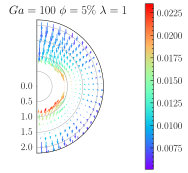
\includegraphics[height=0.3\textwidth]{image/HOMOGENEOUS_NEW/Dist/U_rel_l_1_Ga_100_PHI_5.pdf}
    % \includegraphics[width=5cm]{image/HOMOGENEOUS_NEW/Dist/U_rel_l_10_Ga_100_PHI_10.pdf}
    % \includegraphics[width=5cm]{image/HOMOGENEOUS_NEW/Dist/U_rel_l_1_Ga_100_PHI_10.pdf}
    \caption{Quiver plots of the relative averaged velocity field $\textbf{w}^\text{nst}(\textbf{r},a)$.
    The color map representing the age of the interaction, the early interaction are in dark blue for red for the long time interaction.
    (left) Low \textit{Galileo} number $Ga = 10$.
    (right) High \textit{Galileo} number $Ga = 25$. }
    \label{fig:Why_Ga_matter}
\end{figure}
From \ref{fig:Why_Ga_matter}  we remark that there is a clear asymmetry on the horizontal plan. 
Indeed, as a matter of fact the particles below the test sphere process all vertical velocity. 
One might expect a fore-after symmetry since we are studying pairs of particles. 
Then, how it is that the particle has nearest neighbors coming from the bottom than from the top ? 
First, one has to understand that $P_\text{nst}$ isn't a symmetric function due to the non commutativity of the function $h_{ij}$ in its definition, see \ref{eq:P_nstij}. 
Second, if the neighboring nearest particle is far from the test particle, the chance for this particle to have the test sphere as its nearest neighbor is low. 
Which means that in \ref{fig:Why_Ga_matter} we observe two distinct interaction from the test sphere with its nearest neighbors on the top and on the bottom. 
This disparity is due to the wake of generated by the test particle which tends to attract the particle at the bottom and to push those on the top. 

Following the color map and the vector fields, it can be stated that on average, the nearest neighboring particles approach from the vertical directions and leave
through the sides of the particle of reference. 
In fact, the fields $\textbf{w}^\text{nst}(r, a)$ provide a quantitative averaged representation of what is known as the \textit{Drafting Kissing Tumbling}\citep{fortes1987nonlinear} mechanism even if for $\lambda = 1$ other non-viscous effects may be important \citet{legendre2003hydrodynamic}.

Now let's investigate the disparity between the low and high inertial cases. 
As shown by \ref{fig:Why_Ga_matter} (left), at low \textit{Galileo} number the nearest particle has a tendency to get around the test particle.
Indeed, for high \textit{Galileo} number the relative velocity is nearly null on the sides and below the test particle, whereas for low \textit{Galileo} number the velocity has a clear non-null vertical component. 
Additionally, it is interesting to notice that,  at $\phi = 0.05$ the long interaction was situated on the sides of the test particle, while at $\phi = 0.1$ it is situated in the zone at below right from the test particle. 
The particles situated at the contact of the test particle results from early interaction. 
In brief for $Ga = 10$ it seems that the particle has no difficulty to get around the test particle on the sides, where for a $Ga = 100$ the relative velocity vanish in what seem to be a stagnation zone.


\paragraph*{The volume fraction dependency :}
As it has been observed in both \ref{fig:Pnst_high_Ga} and \ref{fig:Pnst_low_Ga} the effect of particle volume fraction is that it makes the particle distribution more concentrated on the sides of the test particle. 
\begin{figure}[h!]
    \centering
    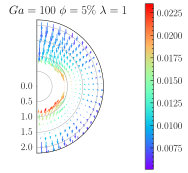
\includegraphics[width=5cm]{image/HOMOGENEOUS_NEW/Dist/U_rel_l_1_Ga_100_PHI_5.pdf}
    \includegraphics[width=5cm]{image/HOMOGENEOUS_NEW/Dist/U_rel_l_1_Ga_100_PHI_10.pdf}
    % \includegraphics[width=5cm]{image/HOMOGENEOUS_NEW/Dist/U_rel_l_10_Ga_100_PHI_10.pdf}
    % \includegraphics[width=5cm]{image/HOMOGENEOUS_NEW/Dist/U_rel_l_1_Ga_100_PHI_10.pdf}
    \caption{Quiver plots of the relative averaged velocity field $\textbf{w}^\text{nst}(\textbf{r},a)$.
    The color map representing the age of the interaction, the early interaction are in dark blue for red for the long time interaction.
    (left) Low \textit{Galileo} number $Ga = 10$.
    (right) High \textit{Galileo} number $Ga = 25$. }
    \label{fig:Why_Phi_matter}
\end{figure}
In \ref{fig:Why_Phi_matter} both graph exhibit the same stagnation zone where the particles result from a long interaction (dark red color) and the particle at contact from short interaction (dark blue color). 
The fact that the interaction at contact is early doesn't mean that the neighboring particles come quickly, it just means that they were already close. 
Additionally, the relative velocity have a high tendency to be oriented downward. 
Overall, the physical interaction doesn't seem to change in this range of volume fraciton. 

\paragraph*{The viscosity ratio dependency :}
Lastly, we now turn our attention to the effect of the viscosity ratio on pair interaction.
The question that we are trying to answer is : why does a smaller viscosity ratio increase the probability density on the horizontal plane ? 
The first point might be explained comparing 2 cases at $Ga = 100$ where we observe a clear difference between the PDF (see \ref{fig:Pnst_high_Ga}) for $\lambda = 1$ and  $\lambda = 10$.
\begin{figure}[h!]
    \centering
    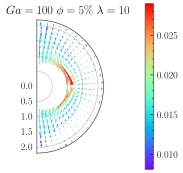
\includegraphics[width=5cm]{image/HOMOGENEOUS_NEW/Dist/U_rel_l_10_Ga_100_PHI_5.pdf}
    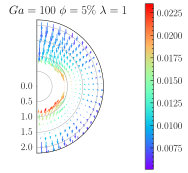
\includegraphics[width=5cm]{image/HOMOGENEOUS_NEW/Dist/U_rel_l_1_Ga_100_PHI_5.pdf}
    % \includegraphics[width=5cm]{image/HOMOGENEOUS_NEW/Dist/F_rel_l_10_Ga_100_PHI_5.pdf}
    % \includegraphics[width=5cm]{image/HOMOGENEOUS_NEW/Dist/F_rel_l_1_Ga_100_PHI_5.pdf}
    \caption{Quiver plots of the relative averaged velocity field $\textbf{w}^\text{nst}(\textbf{r},a)$.
    The color map representing the age of the interaction, the early interaction are in dark blue for red for the long time interaction.
    (left) High viscosity ratio $\lambda = 10$, solid-like particle.
    (right) Low viscosity ratio, $\lambda = 1$ bubble-like particle. }
    \label{fig:Why_l_matter}
\end{figure}
The age is represented by the color map from dark blue for earliest interaction to dark red for the longest interaction. 
To track the course of the averaged path of the nearest particle one has to follow the flow lines $\textbf{w}^\text{nst}$. 
It is then clear from \ref{fig:Why_l_matter} (left) and (right) that the neighboring particle approach on the vertical direction and end up its course on the sides. 
Therefore, it explains why the particles' concentration tends to be higher on the sides as seen in \ref{fig:Pnst_high_Ga}. 
At low $\lambda$ it is seen in \ref{fig:Why_l_matter} (right) that the particle reaches a quasi null relative velocity on the sides. 
Indeed, we identify a clear stagnation zone where the age is maximum and the relative velocity is nearly null. 
On the other hand for $\lambda =10$ the relative velocity on the vicinity of the particle of reference isn't as much as low as for the previous case.
Additionally,  the particles reaches their maximum age while being in contact of the test particle.
This testifies to the interruption of the interaction by another particle. 
Indeed, if the particle in contact of the test sphere suddenly stop being the nearest particle it means that its has been replaced by an other particle. 
In brief, for $\lambda =1$ the particle seem to have lost all of its relative momentum at the end of the interaction leaving them side by side, while when $\lambda =10$ the neighboring particle is still in motion.  
At lower $Ga$ we observe no difference between the velocity fields of two different viscosity ratios. 
At higher volume fraction same comments than above can be made. 
This is consistent with the PDF displayed in \ref{fig:Pnst_low_Ga} where we observed no changes with $\lambda$. 

Overall :
\begin{itemize}
    \item The impact of Galileo is that long interaction arise far from the particle and with no relative velocity, while at low $Ga$ the long interaction can happen on the side.
    \item The volume fraction impact is that long interaction are even further away from the particle. 
    \item The viscosity ratio change the nature of the interaction by rapproching the rad zone. 
    It does mean that there is more close contact long interaction type.
\end{itemize}

The ability of the neighboring particle to stay close to the test particle seems to be the keys to fin out the main difference in behavior between the $\lambda=1$ and  $\lambda = 10$ cases. 
Indeed, as a matter of fact partcile 

\tb{Compare the velocity with \citet{shajahan2023inertial}}

\tb{The asymmetry of the velocity come form the layers in which case bubbles that comming from botton etc is different}

% \subsection{Carrier phase velocity fields}

In the previous section we explained the microstructure formation with kinematic arguments.
Although we indeed provided an explanation the question that arise now id :
Why does the relative velocity behave as such.
The answer might be obtained based on dynamical arguments as it is done often, in such a way we could explain the relative kinematic.
Nevertheless, the dynamical aspect of the interaction is out of the scope of this study and will be treated in a future work. 

Instead, we propose to study the particles averaged wakes to explain the possible difference in interaction between the iso-viscous and viscous droplets cases. 
Again we make use of the nearest particle averaged statistic to compute the carrier fluid phase velocity conditionally on the presence of a particle at \textbf{x}, it reads,
\begin{equation*}
    \textbf{u}^\text{nst}_f P_{nst}(\textbf{x},\textbf{r},t)= 
    \int \sum_{i}^{N_b} \delta(\textbf{x}-\textbf{x}_i(\FF,t))
    h_{i} 
    \textbf{u}_f^0(\textbf{x}+\textbf{r},t,\FF)
    d\mathscr{P} 
\end{equation*}
where $h_{i} = 1$ if the particle $i$ center of mass is the nearest point to the eularian coordinate \textbf{x}+\textbf{r}. 
This velocity fields can be reconstructed as well with our DNS. 
On \ref{fig:stream} we display the reconstructed velocity field $\textbf{u}^\text{nst}_f$ for (left) the iso-viscous case $\lambda =1$ and (right) the viscous droplets' case $\lambda = 10$, for different value of the volume fraction. 
\begin{figure}[h!]
    \centering
    \includegraphics[height=0.4\textwidth]{image/HOMOGENEOUS_NEW/Stream/Stream_PHI_1_Ga_100_l_100}
    \includegraphics[height=0.4\textwidth]{image/HOMOGENEOUS_NEW/Stream/Stream_PHI_1_Ga_100_l_10}
    \includegraphics[height=0.4\textwidth]{image/HOMOGENEOUS_NEW/Stream/Stream_PHI_5_Ga_5_l_100}
    \includegraphics[height=0.4\textwidth]{image/HOMOGENEOUS_NEW/Stream/Stream_PHI_5_Ga_5_l_10}
    \includegraphics[height=0.4\textwidth]{image/HOMOGENEOUS_NEW/Stream/Stream_PHI_20_Ga_100_l_100}
    \includegraphics[height=0.4\textwidth]{image/HOMOGENEOUS_NEW/Stream/Stream_PHI_20_Ga_100_l_10}
    % \includegraphics{image/HOMOGENEOUS_NEW/Stream/Stream_PHI_5_Ga_100_l_1.pdf}
    \caption{Nearest averaged carrier phase velocity fields. }
    \label{fig:stream}
\end{figure}
This velocity field is evaluated at $\textbf{x}+\textbf{r}$ conditioned on the presence of the nearest particle at $\textbf{x}$. 


\tb{compare with \citet{shajahan2023inertial} for explaination }
% 






\subsection{Nearest particles arrangements}
\begin{itemize}
    \item Problematic : "How the particles are arranged relative to each other"
    \item Show : "How to compute the Radial and azimuthal probability density function : $P_{nst}(r)$  and $P_{nst}(\theta)$"
    \item  Conclusion on $P_{nst}(\theta)$ : "We observe that the particles pair becomes oriented with increasing $Ga$ and decreasing volume fraction.
    \item  Conclusion on $P_{nst}(r)$ : "We observe that the particles pair becomes randomly arranged for high $Ga$ but in average they are rather spaced from each other" 
\end{itemize}
\tb{Je me demande si cette section est vraiment utile .... car elle n'apport pas d'explication supplementaire a la drag force ni aux fluctuations, c'est peux être mieux de garder ca pour l'article qui traîte des interactions }

In this section we wish to investigate the particle arrangements and clustering effects. 
As in the previous section we treat this problem with the nearest particle statistics.
We introduce the probability density function defined such that $P_{nst}(\textbf{r})d\textbf{r}$ is the probable number of nearest neighboring particle at a disatnce $\textbf{r}$ from a test particle at $\textbf{r} = 0$. 
Let $\textbf{x}^i(t,\CC)$ and $\textbf{x}^j(\CC,t)$ be the position vector of the particle $i$ and $j$ function of the initial configuration of the flow $\CC$ and the time $t$. 
Then, the nearest pair probability density function is defined such as, 
\begin{equation}
    P_{nst}(\textbf{x},\textbf{r},t)= 
    \int \sum_{i}\delta(\textbf{x}-\textbf{x}^i(\CC,t))
    \sum_{j\neq i}\delta(\textbf{x}+\textbf{r}-\textbf{x}^j(\CC,t)) 
    % \delta(t+a-t_c^{ij}(\CC,t)) 
    h_{ij}(\CC,t) d\mathscr{P} 
    \label{eq:P_nstij}
\end{equation}
with $h_{ij} = 1$ if the particle $j$ is one of the nearest neighbor from the particle $i$, and $h_{ij} = 0$ if it is not. 
Since we model a statistically homogeneous configuration within space and time, the variable \textbf{x} and $t$ are of no interest, thus $P_{nst}(\textbf{x},\textbf{r},t) = P_{nst}(\textbf{r})$. 
\begin{figure}
    \centering
    \begin{tikzpicture}
        \node at (0,0){ \includegraphics[height=0.3\textwidth]{image/HOMOGENEOUS/fDrop/Pnst_theta_mu_r_1_0_Ga_10.pdf} };
        \node at (0.4\textwidth,0){ \includegraphics[height=0.3\textwidth]{image/HOMOGENEOUS/fDrop/Pnst_theta_mu_r_0_1_Ga_10.pdf} };
        \node at (0,-0.3\textwidth){ \includegraphics[height=0.3\textwidth]{image/HOMOGENEOUS/fDrop/Pnst_theta_mu_r_1_0_Ga_75.pdf} };
        \node at (0.4\textwidth,-0.3\textwidth){ \includegraphics[height=0.3\textwidth]{image/HOMOGENEOUS/fDrop/Pnst_theta_mu_r_0_1_Ga_100.pdf} };
        % \node at (0,-0.6\textwidth){ \includegraphics[height=0.3\textwidth]{image/HOMOGENEOUS/fDrop/Pnst_theta_mu_r_1_0_Ga_100.pdf} };
        % \node at (0.4\textwidth,-0.6\textwidth){ \includegraphics[height=0.3\textwidth]{image/HOMOGENEOUS/fDrop/Pnst_theta_mu_r_0_1_Ga_100.pdf} };
    \end{tikzpicture}
    \caption{Probability density function of the nearest particles : $P_{nst}(\theta)$ for different $Ga$ and $\lambda$. 
    Increasing $Ga$ from top to bottom, (left) $\lambda = 1$ (right) $\lambda = 10$. 
    The symbols correspond to different volume fraction ($\bullet$) $\phi = 1\%$, ($\blacktriangle$) $\phi = 5\%$, ($\blacksquare$) $\phi = 10\%$, ($\blacklozenge$) $\phi = 15\%$ and ($\blacktriangleright$) $\phi = 20\%$.
    (dashed lines) empirical formulas }
    \label{fig:P_nst_theta}
\end{figure}
By using polar coordinate such that $d \textbf{r} = r^2 \sin \phi dr d\phi d\theta$ we can further reduce the PDF to the only consideration of the angular dependency $\theta$ or the distance dependency $r$. 
These reduced p.d.f can be computed as follow, 
\begin{align*}
    P_{nst}(r) 
    &= \int_{-\pi/2}^{\pi/2}\int_{0}^{2\theta} P_{nst}(\textbf{x},\textbf{r},t) \sin \theta  d\phi d\theta\\
    P_{nst}(\theta)
    &= \int_{0}^{\infty}\int_{0}^{2\theta} P_{nst}(\textbf{x},\textbf{r},t) r^2  dr d\phi
\end{align*}
\todo{Check if those formulas are true}
Then $P_{nst}(\theta)$ is the probability that the nearest neighbor of a test particle is inclined at an angle $\theta$ relative to the flow direction. 
We observe that the particles pair becomes oriented with increasing $Ga$ and decreasing volume fraction

On \ref{fig:P_nst_theta} we observe that the particles pair becomes oriented with increasing $Ga$ and decreasing volume fraction.
Indeed, we observe a clear peak of $P_{nst}(\theta)$ at $\theta = \frac{\pi}{2}$. 
It seems that this tendency was also reported for spherical bubble in air-water system \citet{bunner2003effect}. 
Additionally, from \ref{fig:P_nst_theta} we can say that the viscosity ratio $\lambda$ seem to prevent the alignment/clustering of particles denoted by the slightly low peak for $\lambda =10$. 
\todo[inline]{Compart the Orientation with bubbly and solid flows \citet{roghair2011drag}}

\begin{figure}
    \centering
    \begin{tikzpicture}
        \node at (0,0){ \includegraphics[height=0.3\textwidth]{image/HOMOGENEOUS/fDrop/Pnst_r_mu_r_1_0_PHI_1.pdf} };
        \node at (0.4\textwidth,0){ \includegraphics[height=0.3\textwidth]{image/HOMOGENEOUS/fDrop/Pnst_r_mu_r_0_1_PHI_1.pdf} };
        \node at (0,-0.3\textwidth){ \includegraphics[height=0.3\textwidth]{image/HOMOGENEOUS/fDrop/Pnst_r_mu_r_1_0_PHI_10.pdf} };
        \node at (0.4\textwidth,-0.3\textwidth){ \includegraphics[height=0.3\textwidth]{image/HOMOGENEOUS/fDrop/Pnst_r_mu_r_0_1_PHI_10.pdf} };
        \node at (0,-0.6\textwidth){ \includegraphics[height=0.3\textwidth]{image/HOMOGENEOUS/fDrop/Pnst_r_mu_r_1_0_PHI_20.pdf} };
        \node at (0.4\textwidth,-0.6\textwidth){ \includegraphics[height=0.3\textwidth]{image/HOMOGENEOUS/fDrop/Pnst_r_mu_r_0_1_PHI_20.pdf} };
    \end{tikzpicture}
    \caption{Radial probability density function : $P_{nst}(r)$ for different $\phi$ and $\lambda$. 
    Increasing $\phi$ from top to bottom, (left) $\lambda = 1$ (right) $\lambda = 10$. 
    The symbols correspond to different Galileo number ($\bullet$) $Ga = 10$, ($\blacktriangle$) $Ga = 25$, ($\blacksquare$) $Ga = 50$, ($\blacklozenge$) $Ga = 75$ and ($\blacktriangleright$) $Ga = 100$.
    (dashed lines) Theoretical formula \ref{eq:P_nst_r}}
    \label{fig:P_nst_r}
\end{figure}
Note that for solid spherical particle in the dilute regime a theoretical formula for $P_{nst}(r)$ can be found assuming completely random distribution and no interactions nor overlap between particles \citep{zhang2021ensemble}, it reads, 
\begin{equation*}
    P_\text{nst}^\text{th}(r) = n_p e^{-4 \pi n_p (r^3 - d^3)/3}.
    \label{eq:P_nst_r}
\end{equation*}
It is evident that all the distribution presented \ref{fig:P_nst_r} have a peak at $r > 1$ where the theoretical formula  predict a peak at $r=1$. 
This is obviously due to the fact that we are in presence of particles interaction which tends to repulse the particles from each others and therefore to shift the distribution to the left. 
What is more interesting is that for $\lambda = 1$ at low volume fraction and high \textit{Galileo} we are able to recover approximately the random particle distribution $P_\text{nst}^\text{th}$ with our numerical results. 
Whereas for $\lambda = 10$ the particle are relatively maintained far from  each other as depicted \ref{fig:P_nst_r}(right). 
We can stipulate that for high viscosity ratio the particles have a tendency to generate more particle fluid mediated interaction as demonstrated by the flow lines \ref{fig:Stream}.


\subsection{Nearest-particle average fluid velocity}
Objectives : 
\begin{itemize}
    \item Problematic "How to analyse the flow around a particle in average"
    \item First : present the averaged the nearest particles' statistics method. And how to compute the nearest averaged velocity fields $\nstavg{\textbf{u}}$.
    \item Present the flowlines and show that for $\phi = 5 \rightarrow 20\%$ we observe that a vertical symmetry arise.
    \item Explain how this field it is related to the velocity fluctuation with \ref{eq:def_uu}
    \item Conclude that these velocity fields represent the PWFs since it represent the mean wakes \citep{du2022analysis}.  
    \item Additionally, some comment can be made regarding the shape of the particle thanks to the contour lines. 
    \item Approach these flow fields by analytical solution of potential flow to obtain an analytical solution for teh reyolds stress. 
\end{itemize}

Presently, we wish to investigate the  averaged flow structure around a fluid particle.
To obtain such a field we make use of the nearest particle statistics recently introduced by \citet{zhang2021stress}. 
We introduce $\nstavg{\textbf{u}}(\textbf{x},\textbf{r})$ as the velocity fields at \textbf{x} knowing there is a particles center of mass located at \textbf{r}.
Additionally, this particle is the nearest particle among all to the point \textbf{x}.  
Formally, this conditional average can be written as, 
\begin{equation}
    \nstavg{\textbf{u}}(\textbf{x},\textbf{r})=\frac{1}{P_{nst}(\textbf{x},\textbf{r})} 
    \int \textbf{u}(\textbf{x},\CC,t) 
    \sum_{\alpha}\delta(\textbf{x}+\textbf{r}-\textbf{x}^\alpha(\CC,t)) h_{\alpha}(\CC,\textbf{x},t) d\mathscr{P} 
    \label{eq:q_nst_avg}
\end{equation}
where $P_{nst}(\textbf{x},\textbf{r})$ is defined as,  
\begin{equation}
    P_{nst}(\textbf{x},\textbf{r})= 
    \int
    \sum_{\alpha}\delta(\textbf{x}+\textbf{r}-\textbf{x}^\alpha(\CC,t)) 
    h_\alpha(\CC,\textbf{x},t) d\mathscr{P}. 
    \label{eq:P_nsti}
\end{equation}
which is the probability of finding a particle center of mass at a distance \textbf{r} from the point \textbf{x} knowing that this particle is the nearest neighbor to the points \textbf{x}. 
The function $h_\alpha$ is defined such that, $h_\alpha = 1/N^p$ if $\alpha$ is the nearest particle to \textbf{x} and $0$ if not, where $N^p$ is the total number of nearest neighbor.
Indeed, the point \textbf{x} at mid-distance from two particles posses two nearest neighbors by definition, thus $N(\textbf{x},\CC,t) = 2$ in this case. 

\todo[inline]{Include the numerical computaiton of $\nstavg{\textbf{u}}$.  }

\ref{fig:Stream} shows the streamline of the field $\nstavg{\textbf{u}}(\textbf{x},\textbf{r})$ for three volume fractions. 
We clearly observe the induced wake of the particles centered at the origin. 

\begin{figure}
    \centering
    \begin{tikzpicture}
        \node (img) at (0,0)  {\includegraphics[height=0.4\textwidth]{image/VALIDATION2.0/Stream/Stream_PHI_20_Ga_10_l_1.pdf}};
        \node (img) at (0.4\textwidth,0)  {\includegraphics[height=0.4\textwidth]{image/VALIDATION2.0/Stream/Stream_PHI_20_Ga_10_l_10.pdf}};
        \node (img) at (0,-0.4\textwidth)  {\includegraphics[height=0.4\textwidth]{image/VALIDATION2.0/Stream/Stream_PHI_20_Ga_100_l_1.pdf}};
        \node (img) at (0.4\textwidth,-0.4\textwidth)  {\includegraphics[height=0.4\textwidth]{image/VALIDATION2.0/Stream/Stream_PHI_20_Ga_100_l_10.pdf}};
        \node (img) at (0,-0.8\textwidth)  {\includegraphics[height=0.4\textwidth]{image/VALIDATION2.0/Stream/Stream_PHI_5_Ga_25_l_10.pdf}};
        \node (img) at (0.4\textwidth,-0.8\textwidth)  {\includegraphics[height=0.4\textwidth]{image/VALIDATION2.0/Stream/Stream_PHI_20_Ga_25_l_10.pdf}};
    \end{tikzpicture}
    \caption{Nearest particle averaged velocity $\nstavg{\textbf{u}}(\textbf{r})$ for  $\phi = 5\%$ and $20\%$.
    Green lines : contour plots of the nearest averaged indicator function $\nstavg{\chi_d}(\textbf{r})$ (it represent the mean shape of the particles)}
    \label{fig:Stream}
\end{figure}
It is evident from these plots that the induced wake is the averaged wake resulting from the averaged translation of the particles. 
And this averaged wake has a tendency to be asymmetrical for low volume fraction and symmetrical for higher ones. 
Additionally, form basic mathematical consideration on the average operators we can demonstrate that :
\begin{multline*}
    \avg{\chi_k \textbf{u}'_k\textbf{u}'_k}(\textbf{x},t)
    + \phi_k \textbf{u}_k\textbf{u}_k
    = \\
    \underbrace{\int (\nstavg{\chi_k \textbf{u}^0_k}  \nstavg{\chi_k \textbf{u}^0_k} / (\nstavg{\chi_k})  P_{nst}(\textbf{x},t,\textbf{r}) d\textbf{r} }_\text{PWFs}
    +\underbrace{\int \nstavg{\chi_k \textbf{v}_k^0\textbf{v}_k^0}  P_{nst}(\textbf{x},t,\textbf{r}) d\textbf{r}}_\text{WIA}
    \label{eq:def_uu}
\end{multline*}
where, $\textbf{v}_k^0  = \textbf{u}_k^0 - \nstavg{\chi_k \textbf{u}^0_k} / \nstavg{\chi_k}$ is the fluctuation of the local velocity relative to the nearest averaged value. 
Consequently, we can decompose the ensemble averaged fluid velocity fluctuations with a first term representing the variance of $\nstavg{\textbf{u}}$ around the mean $\textbf{u}_k$, and a second term representing the variance of $\textbf{u}^0_k$ around the mean  $\nstavg{\textbf{u}}$. 

There are two phenomena causing velocity fluctuations in the liquid:
the agitation resulting from wakes and their collective interactions [wake-induced agitation (WIA)], and the non-turbulent fluctuations resulting from averaged wakes and potential flows around bubbles [potential flow and averaged wake fluctuations (PWFs)].
As a matter of fact in the phase space of $\nstavg{\textbf{u}}(\textbf{r})$ the bubble is fixed at the origin thus we recover the velocity fields representing what is called the PWFs. 
In their study \citet{du2022analysis} carry out transient simulation with fixed particles to recover the PWFs components here we show that a single simulation permit us to recover WIA and PWFs by the mean of the nearest particles' statistics. 

\todo[inline]{make the link with drag force/drag coef  \citet{dandy1989buoyancy}}
\todo[inline]{make the link with velocity fluctuation \citet{almeras2021statistics}}





o

\section{Conclusion}
\section{Conclusion}

% \citet{einstein1905neue,taylor1932viscosity} demonstrated how the first moment of the hydrodynamic forces (Stresslet) applied on a particle immersed in pure linear flow induced an additional viscosity to the mixture. 
% Later~\citet{zhang1994ensemble,lhuillier1996contribution,jackson1997locally,zhang1997momentum} demonstrated that the second moment of forces were also contributing to the stresses inducing a non-newtonian behaviors, even in the Stokes and dilute limit.  

In this work we computed the moments of force on the surface of a test droplet in the situation of uniform relative motions between the droplet and the continuous phase. 
We considered low but finite Reynolds number $Re$. 
The averaged first moment of force is given by~\ref{eq:forces_reformulated2_avg}, scales as $O(\rho_f \phi u_r^2)$, hence contributing to the averaged Stress of the suspension on the same ground as  \citet{einstein1905neue} or \citep{taylor1932viscosity} correction to the viscosity of the mixture. 
In a lesser extend the inertial part of the second moment also contribute to the Rheology. 
This first point constitutes the main result of the paper. 

Others important conclusion reached through this work includes: a general reciprocal formula to derive the forces and moments on droplets, and the explicit appearing of the velocity variance term in the drag force term. 







\appendix
%\section{Statistical convergence and mesh independence studies}
\section{Numerical validations}
\label{ap:validation}
\section{Numerical validations}
\label{ap:validation}
The \texttt{Basilisk} code has been validated numerous times in previous numerical studies. 
Especially, we can cite the recent studies of \citet{innocenti2020direct} and \citet{hidman2023assessing} which both performed DNS of rising suspensions of bubbles. 
Nevertheless, in this work we investigate specific statistical distributions,
and we make use of a multi-VoF method to avoid droplets coalescence, therefore a meticulous validation of the DNS is in order. 
We start by presenting a brief comparison with the reference DNS of \citet{esmaeeli1999direct}. 
Afterward we present a study focusing on the interface kinematics where we compare our DNS with the experimental results of \citet{mohamed2003drop} to show that the multi-VoF method indeed captures the physics of two colliding interfaces without resolving the flow within the separating film. 
Once the mesh and the physics are validated, a study on the convergence of the statistics is presented. 

\subsection{Ordered array of buoyant bubbles}

From our knowledge, no simulations nor experimental results have been carried out for rising buoyant viscous droplets. 
Therefore, we reproduced instead the ordered array simulation of \citet{esmaeeli1999direct} with \texttt{Basilisk} to validate the mesh resolution of our DNS.  
It consists in a 3-D buoyant ordered rising array of bubbles. 
In our notation the flow parameters of the simulation read 
\begin{align*}
    \lambda = 10,
    && \zeta = 10,
    && Bo = 1.8,
    && Ga = 28.37,
    && \phi = 0.125.
\end{align*}
\begin{figure}[h!]
    \centering
    \includegraphics[height = 0.3\textwidth]{image/VALIDATION2.0/Loisy/Re.pdf}
    \caption{Time evolution of the Reynolds number based on the instantaneous volume averaged drift velocity, $Re_d(t) = \rho_fU _dd /\mu_f$, with $U_d(t)$ the drift velocity defined as $U_d = |\textbf{u}_d - \textbf{u}|$ with $\phi = 0.1256$, $\zeta =\mu_r =10$ and $Ga = 29.9$. $\textbf{u}_d$ and $\textbf{u}$ represent the volume-averaged velocities of the dispersed phase and the bulk, respectively, at time $t$.}
    %$\textbf{u}_d$ and $\textbf{u}$ are the average of the dispersed phase velocity and bulk velocity at time $t$ respectively.}
    \label{fig:ordered_array}
\end{figure}
\ref{fig:ordered_array} displays our numerical simulation against the original result of \citet{esmaeeli1999direct}.
We observe very good agreements between both studies for all mesh resolutions.
Additionally, we displayed the results of \citet{innocenti2020direct} for $d/\Delta = 20$ to point out a divergence with our results at the same mesh resolution.  
Both our simulations and the one of \citet{innocenti2020direct} have been carried out with the  \texttt{Basilisk} code. 
The cause of this difference is in fact due to a different method of interpolation used for the viscosity coefficient $\mu$. 
We used an arithmetic mean whereas \citet{innocenti2020direct} used an 
harmonic mean.
As a matter of fact in this regime the arithmetic mean, which will be used in this work, permits us to reach a faster convergence. 
Overall these results indicate that the criterion $d/\Delta = 20$ seems sufficient.%, which is consistent with the aforementioned studies.


\subsection{Drop impact on a liquid-liquid interface}

In this section we investigate in more detail the physics behind the multi-VoF method. 
We need to verify if we accurately capture the physics of the droplets interfaces despite the fact that we do not resolve accurately the film between two droplets. 
Following \citet{balcazar2015multiple} we reproduced the experiment of drop impact on a liquid–liquid interface carried by \citet{mohamed2003drop} but with the \texttt{Basilisk} code. 
This experiment consists in letting a drop fall into a pool of the same fluid as the drop. 
All along the experiment the interfaces of the droplets and the pool are tracked. 
In our notation the dimensionless parameters read 
\begin{align*}
    Ga = 71.02 
    && Bo = 6.40
    && \lambda = 0.33
    && \zeta = 1.189
\end{align*}
Following \citet{mohamed2003drop} we defined the dimensionless time $t / t_i = t U_i(t) /d$ where $U_i(t)$ is droplet velocity at $t<0$ and where $t=0$ is the time of impact. 
Regarding the geometry of the problem we sketched in \ref{fig:schemeLong} the initial position of the droplet in the computational domain.
Additionally, we display on \ref{fig:schemeLong} a snapshot of the numerical domain were we see the drop colliding the pool interface.
The drop and the pool do not merge since we use the multi-VoF method. 
Note that in the experiment the drop does not merge with the pool either.
This enables us to represent with the DNS a physical situation where the interfaces do not coalesce, but where we use a grid resolution of $d/\Delta = 20$ which is of course not sufficient to resolve the flow inside the film. 
\begin{figure}[h!]
    \centering
    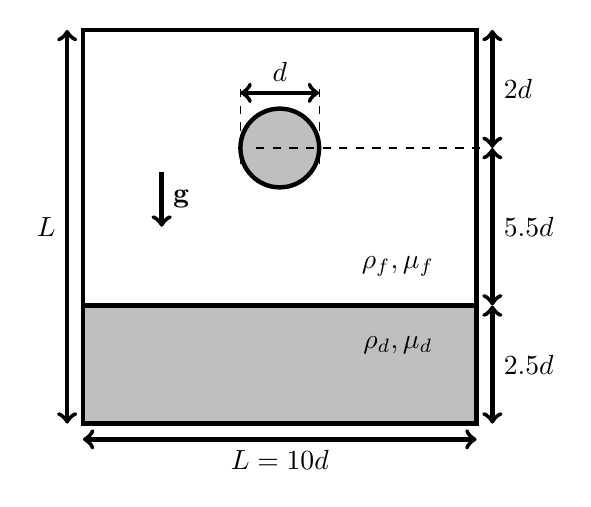
\begin{tikzpicture}[ultra thick]
        \draw (0,0) rectangle (5,5);
        \draw[fill=gray!50] (0,0) rectangle (5,1.5);
        \draw[fill=gray!50] (2.5,3.5) circle (0.5);
        \draw[<->](0,-0.2) --++ (5,0)node[midway,below]{$L  = 10 d$};
        \draw[<->](-0.2,0) --++ (0,5)node[midway,left]{$L$};
        \draw[<->](5.2,0) --++ (0,1.5)node[midway,right]{$2.5 d$};
        \draw[<->](5.2,1.5) --++ (0,2)node[midway,right]{$5.5 d$};
        \draw[<->](5.2,3.5) --++ (0,1.5)node[midway,right]{$ 2d$};
        \draw[dashed,thin](2.2,3.5) --++ (2.9,0);
        \draw[dashed,thin](2.2,3.5) --++ (2.9,0);
        \draw[->](1,3.2) --++ (0,-0.7)node[midway,right]{$\textbf{g}$};
        \draw[<->](2,4.2) --++ (1,0)node[midway,above]{$d$};
        \draw[thin,dashed](2,3.3) --++ (0,1);
        \draw[thin,dashed](3,3.3) --++ (0,1);
        \node (a) at (4,2){$\rho_f, \mu_f$};
        \node (a) at (4,1){$\rho_d, \mu_d$};
    \end{tikzpicture}
    \includegraphics[height = 0.4\textwidth]{image/VALIDATION2.0/Longmire/IMG/image-079.png}
    \caption{(left) Sketch of the computational set up at the initial time. 
    (right) Snapshot of the computational domain after the collision, with the pool interface represented in gray.
    The background color represents the velocity field magnitude, which is undisturbed, indicating a large enough domain. }
    \label{fig:schemeLong}
\end{figure}
\begin{figure}[h!]
    \centering
    \includegraphics[height = 0.3\textwidth]{image/VALIDATION2.0/Longmire/Re.pdf}
    \includegraphics[height = 0.3\textwidth]{image/VALIDATION2.0/Longmire/Dist.pdf}
    \caption{(left) Time evolution of the Reynolds number based on the droplet velocity, $Re(t) = \rho_fU d /\mu_f$ as a function of the dimensionless time, (+) numerical results of  \citet{balcazar2015multiple} (right)  position of the interfaces, ($\bullet$) top droplet surface, ($+$) bottom droplet surface, (x) pool surface. (Symbols) Experimental results of \citet{mohamed2003drop} (solid line) present numerical simulations with $d/\Delta = 20$. }
    \label{fig:resultslong}
\end{figure}
\ref{fig:resultslong} represents the comparison between our results and the experiment of \citet{mohamed2003drop} (right) and the numerical simulation of \citet{balcazar2015multiple} (left). 
The time-dependent Reynolds number as well as the interfaces positions are shown to closely match both the numerical and experiential results. 
From the very good agreement we conclude that the kinematics are well-represented even during contact for a mesh resolution of $d/\Delta = 20$.

\subsection{Mesh independence and statistical convergence for random arrays of drops}

Even though the aforementioned studies carried validations of the \texttt{Basilisk} code for rising droplets or bubbles, almost all of them considered isolated droplets or bubbles as the only validation case. 
To the author's knowledge, to this date no published study has presented a mesh independence study for random arrays of droplets or bubbles of this scale. 
As particle interactions and higher \textit{Galileo} numbers may be more challenging to model, it is primordial to investigate the mesh independence of the DNS that are carried in this work. 
In this objective we performed a DNS of a random array of $N_b=125$ droplets, with the following parameters
\begin{align*}
    \lambda = 10,
    && \zeta = 1.11,
    && Bo = 0.2,
    && Ga = 100,
    && \phi = 0.1,
    && N_b =125,
\end{align*}
with mesh resolutions of $d/\Delta = 5,\; 10,\; 18,\; 37$. 
This set of parameters have been selected following these arguments :
A viscosity ratio $\lambda = 10$ induces more vorticity at the droplets interfaces in contrast with the $\lambda = 1$ cases. 
For high inertia regimes ($Ga = 100$) the boundary layers at the droplet interfaces require the fine grid to be resolved compared to the low inertia cases. 
At $\phi = 0.1$, numerous interactions of droplets are present, implying that the good modeling of the liquid films between interfaces becomes predominant on the overall hydrodynamic, this also requires a good mesh resolution. 
% Additionally, the lower \textit{Bond} number employed here ($Bo=0.2$ instead of $Bo =0.5$) requires a higher mesh quality as well. 
For these reasons, we suppose that this case might require the finest grid among all other cases presented in this study. 
Based on this remark we can assume that if this case is mesh independent, then all cases from \ref{tab:simulations} are equally validated. 

Let us first verify the independence of the drift velocity on the mesh resolution. 
\begin{figure}[h!]
    \centering
    \includegraphics[height = 0.3\textwidth]{image/HOMOGENEOUS_NEW/VAL/tr.pdf}
    \includegraphics[height = 0.3\textwidth]{image/HOMOGENEOUS_NEW/VAL/Re.pdf}
    \caption{
        (left) Running average of the trace of $\textbf{R}$ as a function of the dimensionless time $t \sqrt{d/g}$. 
        (right) Running average of the Reynolds number based on the instantaneous volume-averaged relative velocity, $Re(t) = \rho_f U d /\mu_f$, with $U(t) = |\textbf{u}_d - \textbf{u}_c|$ for $\phi = 0.1$, $Ga=100$ and $\lambda =10$. 
        $\textbf{u}_d$ and $\textbf{u}_c$ represent the volume-averaged velocities of the dispersed phase and the continuous phase, respectively, at the dimensionless time $t \sqrt{d/g}$.
        %$\textbf{u}_p$ and $\textbf{u}_f$ are the particle and fluid phase volume averaged velocity at time $t$.
        In the legend we display the value of the mesh resolution. 
    }
    \label{fig:Re}
\end{figure}
In \ref{fig:Re} we display the running-averaged drift velocity as a function of time, for four mesh resolutions. 
The results are not as independent of the mesh resolution as the ordered array validation presented above. 
Indeed, we observe a difference of the rising Reynolds number of about $5\%$ between the $d/\Delta = 18$ and $d/\Delta = 37$ cases which is notable.
We recall that this $5\%$ error will eventually be lower for all other cases. 
The good agreement between the case  $d/\Delta = 10$ and $d/\Delta = 18$ is partially fortuitous.


% In \ref{fig:Re} (right) we display the running-averaged drift velocity as a function of time, for five mesh resolutions. 
% The results are not as independent of the mesh resolution as the ordered array validation presented above. 
% Indeed, we observe a difference of the rising Reynolds number of about $ 3\%$ between the $d/\Delta = 25$ and $d/\Delta = 60$ cases which is notable.
% We recall that this $3\%$ error will eventually be lower for all other cases. 

Now, let us turn our attention to \ref{fig:Re} (left), where we display the running average of $\text tr(\textbf{R})/r_m^2$ for different mesh resolutions.  
This figure validates two important points. 
First, we notice that the average of $\text tr(\textbf{R})/r_m^2$ appears well-converged at large $t\sqrt{d/g}$. 
This indicates that we have gathered a sufficient number of statistics to obtain accurate results. 
Secondly, it is found that the four cases converge approximately to the same value at large  $t\sqrt{d/g}$, implying that this quantity is also mesh-independent. 

\subsection{ Domain size independence study}

As discussed in the main text, the length scale of the distance between the particle layers is of the same order as the domain size. 
This raises an important question: Is the observed microstructure a physical phenomenon, or merely an artifact of the domain's size?
To address this, we conducted a DNS of a random array of $N_b=800$ droplets with a domain size of $\mathcal{L}/d = 20$. With the following dimensionless parameters:
\begin{align*}
    \lambda = 1,
    && \zeta = 1.11,
    && Bo = 0.5,
    && Ga = 80,
    && \phi = 0.05. 
\end{align*}
Note that the \textit{Galileo} number and the \textit{Bond} number are slightly different than in the original set of DNS due to numerical constraints.
We expect that these changes are not significant, so that the comparison remains valuable.


In \ref{fig:Pnst_large_domain} we compare the distribution $P_\text{nst}$ from the current case with $N_b =800$ droplets to the dataset used in this study with $N_b = 125$ droplets.
A good agreement is observed between the two distributions, although slight differences are noticeable.
These differences could be due to the different \textit{Galileo} numbers used in the larger simulation.
Nevertheless, the anisotropic behavior of $P_\text{nst}$ appears to be preserved between these two DNS.   
\begin{figure}[h!]
    \centering
    \includegraphics[height=0.205\textwidth]{image/HOMOGENEOUS_NEW/Dist/Pnst_l_1_Ga_100_PHI_0_05.pdf}
    \includegraphics[height=0.205\textwidth]{image/HOMOGENEOUS_final/Dist/Pnst_l_1_Ga_80_PHI_0_05.pdf}
    \caption{Histogram of the normalized function $P_\text{nst}$ at high inertia $Ga = 100$.
    The color map represents the values of the nearest pair distribution function. %of $P_\text{nst}$.
    The origin corresponds to the position of the \textit{\textit{test particle}}.
    The dimensionless radial and azimuthal coordinates, $|\textbf{r}|/d$ and $\theta$, correspond to the nearest neighbor position.
    The vertical direction corresponds to the flow direction, which is also the axis of symmetry for $P_\text{nst}$.
    (left) Original DNS with $N_b =125$ droplets.
    (right) Reference DNS with $N_b = 800$ droplets.}
    \label{fig:Pnst_large_domain}
\end{figure}
To provide a qualitative visualization of the system behavior, we displayed in \ref{fig:images_deux} a snapshot from both DNS. 
\begin{figure}[h!]
    \centering
    \includegraphics[width=0.45\textwidth]{image/HOMOGENEOUS_NEW/P_PHI_5_l_10_Ga_100.png}
    \includegraphics[width=0.45\textwidth]{image/HOMOGENEOUS_final/Ga_80_phi_005_l_1.png}
 %    \includegraphics[width=0.45\textwidth]{image/HOMOGENEOUS_NEW/Ga_100_phi_005_l_10.png}
    \caption{Snapshot of a simulation at $t^* = 150$ for $\phi=0.05$.
    Color map : values of the vertical component of the velocity, field on the vertical plane defined by the equation $z=0$. 
    (left)  Tipical DNS used in this study  with $\lambda = 1$ and $N_b = 125$ droplets.
    (right) A larger DNS with same $\phi$ and  $\lambda$ but with $N_b = 800$ droplets.
    }
    \label{fig:images_deux}
\end{figure}
We can observe that the DNS with $N_b = 800$ droplets also exhibits layers and clusters of droplets, similar to the original simulation. 
At this stage, we have not delved into quantitative analysis to verify if the distance between layers is consistent across both sets of simulations. 

Overall, we conclude that the domain size used in this work, $\mathcal{L}/d = 10$, is sufficient. 
Indeed, The distribution $P_\text{nst}$ remains similar in the larger domain (with $\mathcal{L}/d = 20$), and the microstructure displays the same types of particle layers and clusters.
% 
% \subsection{Statistical and mesh independence study}
\tb{Should i put the number of realization is abs $\omega$}

In the aim of providing accurate closure terms it is of primary importance to verify the well convergence of the mean quantities, either by varing the mesh definition domain size and duration of simulation.
To tackle this problem we carried out four simulation with 125 rising droplets with different mesh definition. 
The flow parameters for this validation read as,  
\begin{align*}
    \mu_r = 0.1,
    && \rho_r = 1.11,
    && Bo = 1,
    && Ga = 75,
    && \phi = 0.1,
    && N_b =125. 
\end{align*}
Note that in these simulations we used a number of $125$ droplets.  
In \ref{ap:A} we give more details on this choice and show that for our concerns it is a sufficient number of droplets. 

\ref{fig:Re_and_Tc}(left) display the cumulative mean of the vertical Reynolds number based on the drift velocity, namely,
\begin{equation}
    \widetilde{Re}(t)
    = \frac{\rho_f d}{\mu_f t}\int_{t_0}^{t_0+t} \left(\Xavg{\textbf{u}^0_d} -  \Xavg{\textbf{u}_c^0}\right)dt'
\end{equation}
\tb{ time average and volume average}
where $t_0$ is the starting sampling time. 
We remark a significant dependence of $\tilde{Re}$ with the mesh definition in contrast to the latter study (see \ref{fig:ordered_array}). 
It is hard to distinguish the cause of this difference, if it is not just because of the presence of interaction between droplets. 
Anyhow, we reach mesh independent results for $d/\Delta \geq 30$ in agreements with the recent studies of \citet{loisy2017buoyancy} \citet{zhang2021direct} for low inertial bubbly flows.
Also, $\widetilde{Re}$ reaches a constant values from $t^* = 50$. 
This is true for all mesh definition.  
Consequently, we reached an accurate time convergence for the rising velocity. 
\begin{figure}[h!]
    \centering
    % \includegraphics[height = 0.3\textwidth]{image/VALIDATION2.0/fCA/Re.pdf}
    \includegraphics[height = 0.3\textwidth]{image/VALIDATION2.0/fCA/Recum.pdf}
    \includegraphics[height = 0.3\textwidth]{image/VALIDATION2.0/fCA/Tcum.pdf}
    % \includegraphics[height = 0.35\textwidth]{image/VALIDATION2.0/fPA/Tcum.pdf}
    \caption{(left) Cumulative mean of the volume averaged Reynolds number along the simulation time based on the drift velocity $U = \textbf{u}_p - \textbf{u}_c$, with $\phi = 0.1$, $\rho_r = 1.11$, $ \mu_r =0.1$ and $Ga = 29.9$ and $N_b = 125$.
    (right) Cumulative mean of the fluid Reynolds stress tesor. }
    \label{fig:Re_and_Tc}
\end{figure}

The well convergence of the rising velocity doesn't guarantee a statistical nor a mesh convergence for finer quantities such as the pseudo-turbulent kinetic energy. 
Therefore, we provide on \ref{fig:UpUp} (left) the running average of the fluid phase pseudo-turbulent energy. 
Similarly, \ref{fig:UpUp} (right) represent the particle center of mass pseudo-turbulent kinetic energy. 
\begin{figure}[h!]
    \centering
    \includegraphics[height = 0.3\textwidth]{image/VALIDATION2.0/fCA/Tcum.pdf}
    \includegraphics[height = 0.3\textwidth]{image/VALIDATION2.0/fPA/Tcum.pdf}
    \caption{(left) Cumulative mean of the volume averaged granular temperature along the simulation time based on the drift velocity $U = \textbf{u}_p - \textbf{u}_c$, with $\phi = 0.1$, $\rho_r = 1.11$, $ \mu_r =0.1$ and $Ga = 29.9$ and $N_b = 125$.
    (right) Cumulative mean of the dimensionless particle-fluid-particle stress horizontal component tensor. }
    \label{fig:UpUp}
\end{figure}
Both figure exhibit well converged data. 
Interestingly, $\widetilde{K}_c$ and $\widetilde{K}_\alpha$ reach a constant value at $t^* = 200$ which is four time greater than for $\widetilde{Re}$.


\tb{this convergence can be compared to Loisy studies}
\tb{Cite and compare to Berner and \citet{bunner2002dynamics} which found that Nb > 12 is sufficient \citet{roghair2011drag}}
Now, let's investigate the required number of droplets per domain, $N_b$, and the minimum definition of cells per diameter of droplets $\delta$.  
\tb{Include bibliography and expectation here \ldots}
For this investigation we kept the physical parameters presented in the same section and made a double parametric analysis over $N$ and $\delta$. 
We carried out simulations for $N = 2, 3, 4, 5, 6, 7$, and for a number of cells $10 <\delta < 40$. 
In Basilisk the mesh definition is defined by a power of two, consequently depending on the size of the domain (which is fixed to keep a $\phi$ constant) the $\delta$ parameter is fixed at a power of 2 close. 
\begin{figure}[h!]
    \centering
    \includegraphics[height= 0.3\textwidth]{image/VALIDATION/N_and_delta/DUd.pdf}
    \includegraphics[height= 0.3\textwidth]{image/VALIDATION/N_and_delta/PHI.pdf}
    \caption{(left) Averaged Reynolds number based on the drift velocity.
            (right) Dispersed phase volume fraction at the end of each simulation.
            The text on the side of the points is $\delta$.
            N correspond to $N = N_b^3$. }
    \label{fig:VALIDATION_Nd_1}
\end{figure}
\ref{fig:VALIDATION_Nd_1}(left), illustrate clearly that the drift velocity is independent of the parameters $N_b$ and $\delta$, for $N >4$. 
On the other hand, \ref{fig:VALIDATION_Nd_1}(right), show that the volume fraction of the dispersed phase is lower for the low defined grid (red dots), due to a loss of volume during the simulation.
This doesn't mean that the solver isn't volume conservative. 
In fact, it is fund to be due to the \href{http://basilisk.fr/sandbox/fintzin/Rising-Suspension/no-coalescence.h}{no-coalescence.h} which generate fragment into the numerical domain, fragment which are deleted in the long run. 
\begin{figure}[h!]
    \centering
    \includegraphics[height= 0.3\textwidth]{image/VALIDATION/N_and_delta/PA_UpUp.pdf}
    \includegraphics[height= 0.3\textwidth]{image/VALIDATION/N_and_delta/Mh.pdf}
    \caption{(left) Fluids phase averaged fluctuation tensor.
            (right) Particular average of the first moment tensor, where $F_g$ is the buoyancy force applied on one droplet. 
            The numerical values displayed alongside the dots are the number of cells per diameter.}
    \label{fig:VALIDATION_Nd_2}
\end{figure}
Now, let's look at the behavior of more \textit{complicated} closure terms. 
\ref{fig:VALIDATION_Nd_2}(left) demonstrate that the vertical component of the pseudo turbulent tensor is parameter independent rather early, independently of the grid definition. 
This fact is rather surprising but note that the standard deviation is quite high for small domain. 
On \ref{fig:VALIDATION_Nd_2}(right), we can examine the vertical component of the first moment closure term. 
It is found to be constant for all $N$, but rather inaccurate for coarse grids. 
Which makes sens since the first moment results from a local calculation of the stress over a droplet volume, unlike the other quantities which results from the averaged center of mass velocity of a droplet. 

As we have shown, the quantities presented converge for a number of droplets equivalent to $N = 4$ and $\delta = 25$. 
Thus, we validate our simulation in space, i.e. we made sure that our domain were wide enough to minimize the influence of the periodicity on our results, and in mesh definition. 
Nevertheless, at it is the number of realization that matter when carrying a particular average, it is interesting to look at the duration of the simulation.


The last validation that we must expose is the convergence with the relative properties. 
Indeed, the film definition might change interaction properties such that the particle normal approach $\textbf{w}_n(a)$. 
\begin{figure}[h!]
    \centering
    \includegraphics[height=0.3\textwidth]{image/VALIDATION2.0/Hnst/ur_a_ndc_35_Ga_75.pdf}
    \caption{Normal approach Nearest particle velocity for different $Ga$. 
    We can see that for $\delta = 29,60$ we obtain the same results.}
\end{figure}



\section{Age distribution at low \textit{Galileo} numbers}
\label{ap:age}

We provide additional age distribution for low \textit{Galileo} number to support the argumentation in the body of the text. 
\begin{figure}[h!]
    \centering
    \includegraphics[height = 0.3\textwidth]{image/HOMOGENEOUS_NEW/Dist/Pa_l_1_Ga_10.pdf}
    \includegraphics[height = 0.3\textwidth]{image/HOMOGENEOUS_NEW/Dist/Pa_l_10_Ga_10.pdf}
    \caption{(left) Age distribution at $\lambda = 10$ and $Ga = 10$ for : (solid line) $\phi = 0.2$; (dash dotted line) $\phi = 0.1$; (dashed line) $\phi =0.05$; (dotted line) $\phi = 0.01$. 
    (right) Mean dimensionless age in terms of the volume fraction $\phi$ for : 
    ($\bullet$) $Ga=1$; ($\blacktriangle$) $ Ga = 10$; ($\blacksquare$) $Ga = 50$ ($\blacklozenge$) $Ga =100$.
    The age and $\tau_a$ are made dimensionless with $U/d$ where $U$ is the drift-velocity between the dispersed and continuous phase.  }
    \label{fig:age_picture}
\end{figure}

\bibliography{Bib/bib_bulles.bib}




\end{document}

